% This is "sig-alternate.tex" V2.0 May 2012
% This file should be compiled with V2.5 of "sig-alternate.cls" May 2012
%
% This example file demonstrates the use of the 'sig-alternate.cls'
% V2.5 LaTeX2e document class file. It is for those submitting
% articles to ACM Conference Proceedings WHO DO NOT WISH TO
% STRICTLY ADHERE TO THE SIGS (PUBS-BOARD-ENDORSED) STYLE.
% The 'sig-alternate.cls' file will produce a similar-looking,
% albeit, 'tighter' paper resulting in, invariably, fewer pages.
%
% ----------------------------------------------------------------------------------------------------------------
% This .tex file (and associated .cls V2.5) produces:
%       1) The Permission Statement
%       2) The Conference (location) Info information
%       3) The Copyright Line with ACM data
%       4) NO page numbers
%
% as against the acm_proc_article-sp.cls file which
% DOES NOT produce 1) thru' 3) above.
%
% Using 'sig-alternate.cls' you have control, however, from within
% the source .tex file, over both the CopyrightYear
% (defaulted to 200X) and the ACM Copyright Data
% (defaulted to X-XXXXX-XX-X/XX/XX).
% e.g.
% \CopyrightYear{2007} will cause 2007 to appear in the copyright line.
% \crdata{0-12345-67-8/90/12} will cause 0-12345-67-8/90/12 to appear in the copyright line.
%
% ---------------------------------------------------------------------------------------------------------------
% This .tex source is an example which *does* use
% the .bib file (from which the .bbl file % is produced).
% REMEMBER HOWEVER: After having produced the .bbl file,
% and prior to final submission, you *NEED* to 'insert'
% your .bbl file into your source .tex file so as to provide
% ONE 'self-contained' source file.
%
% ================= IF YOU HAVE QUESTIONS =======================
% Questions regarding the SIGS styles, SIGS policies and
% procedures, Conferences etc. should be sent to
% Adrienne Griscti (griscti@acm.org)
%
% Technical questions _only_ to
% Gerald Murray (murray@hq.acm.org)
% ===============================================================
%
% For tracking purposes - this is V2.0 - May 2012

\documentclass{sig-alternate}

\usepackage{import}

\usepackage{caption}
\usepackage{subcaption}

\usepackage{algorithmic}
\usepackage{algorithm}

\usepackage{array}

\usepackage{graphicx}
\usepackage{epstopdf}

\usepackage{color}

\usepackage[english]{babel}
\usepackage{adjustbox}
%\usepackage[table]{xcolor}
\usepackage{color, colortbl}
\definecolor{high}{rgb}{0.7,.85,.85}
\usepackage{cite}
%\usepackage[sort]{natbib}
\usepackage{mathtools}

% Fancy itemized lists
\usepackage{enumitem}


\DeclarePairedDelimiter{\ceil}{\lceil}{\rceil}
\DeclarePairedDelimiter{\floor}{\lfloor}{\rfloor}

\graphicspath{{./figures/overview/}}

\renewcommand{\algorithmicrequire}{\textbf{Input:}}
\renewcommand{\algorithmicensure}{\textbf{Output:}}



% Datasets
\newcommand{\blogcatalog}{\textsc{BlogCatalog}}
\newcommand{\flickr}{\textsc{Flickr}}
\newcommand{\cora}{\textsc{Cora}}
\newcommand{\citeseer}{\textsc{Citeseer}}
\newcommand{\pokec}{\textsc{Pokec}}
\newcommand{\youtube}{\textsc{YouTube}}

\newcommand{\todo}[1]{{\small\color{red}{\bf #1}}}


% Algorithms
\newcommand{\ouralgorithm}{\textsc{DeepWalk}}

\newcommand{\socdimL}{\text{SpectralClustering}}
\newcommand{\socdimB}{\text{Modularity}}
\newcommand{\socdimA}{\text{EdgeCluster}}
\newcommand{\wvrn}{\text{wvRN}}

% Fancy math symbols
\newcommand{\Laplacian}{\widetilde{\mathcal{L}}}
\newcommand{\comment}[1]{}
% Fancy hypination rules
%\hyphenation{Spectral-Clustering}

\begin{document}
%
% --- Author Metadata here ---
%\conferenceinfo{WOODSTOCK}{'97 El Paso, Texas USA}
%\CopyrightYear{2007} % Allows default copyright year (20XX) to be over-ridden - IF NEED BE.
%\crdata{0-12345-67-8/90/01}  % Allows default copyright data (0-89791-88-6/97/05) to be over-ridden - IF NEED BE.
% --- End of Author Metadata ---

\title{DeepWalk: 
%Better Network Classification through Social Representation Learning
Online Learning of Social Representations
%\titlenote{(Produces the permission block, and
%copyright information). For use with
%SIG-ALTERNATE.CLS. Supported by ACM.}
}
%\subtitle{[Extended Abstract]
%\titlenote{A full version of this paper is available as
%\textit{Author's Guide to Preparing ACM SIG Proceedings Using
%\LaTeX$2_\epsilon$\ and BibTeX} at
%\texttt{www.acm.org/eaddress.htm}}}

%
% You need the command \numberofauthors to handle the 'placement
% and alignment' of the authors beneath the title.
%
% For aesthetic reasons, we recommend 'three authors at a time'
% i.e. three 'name/affiliation blocks' be placed beneath the title.
%
% NOTE: You are NOT restricted in how many 'rows' of
% "name/affiliations" may appear. We just ask that you restrict
% the number of 'columns' to three.
%
% Because of the available 'opening page real-estate'
% we ask you to refrain from putting more than six authors
% (two rows with three columns) beneath the article title.
% More than six makes the first-page appear very cluttered indeed.
%
% Use the \alignauthor commands to handle the names
% and affiliations for an 'aesthetic maximum' of six authors.
% Add names, affiliations, addresses for
% the seventh etc. author(s) as the argument for the
% \additionalauthors command.
% These 'additional authors' will be output/set for you
% without further effort on your part as the last section in
% the body of your article BEFORE References or any Appendices.

\numberofauthors{3} %  in this sample file, there are a *total*
% of EIGHT authors. SIX appear on the 'first-page' (for formatting
% reasons) and the remaining two appear in the \additionalauthors section.
%
\author{
% You can go ahead and credit any number of authors here,
% e.g. one 'row of three' or two rows (consisting of one row of three
% and a second row of one, two or three).
%
% The command \alignauthor (no curly braces needed) should
% precede each author name, affiliation/snail-mail address and
% e-mail address. Additionally, tag each line of
% affiliation/address with \affaddr, and tag the
% e-mail address with \email.
%
% 1st. author
\alignauthor
       Bryan Perozzi\\
\affaddr{Stony Brook University}\\
\affaddr{Department of Computer Science}\\
% 2nd. author
\alignauthor
	   Rami Al-Rfou\\
\affaddr{Stony Brook University}\\
\affaddr{Department of Computer Science}\\
% 3rd. author
\alignauthor 
	   Steven Skiena\\
\affaddr{Stony Brook University}\\
\affaddr{Department of Computer Science}\\
\end{tabular}\newline\begin{tabular}{c}
\{bperozzi, ralrfou, skiena\}@cs.stonybrook.edu\\
}
% There's nothing stopping you putting the seventh, eighth, etc.
% author on the opening page (as the 'third row') but we ask,
% for aesthetic reasons that you place these 'additional authors'
% in the \additional authors block, viz.
%\additionalauthors{Additional authors: John Smith (The Th{\o}rv{\"a}ld Group,
%email: {\texttt{jsmith@affiliation.org}}) and Julius P.~Kumquat
%(The Kumquat Consortium, email: {\texttt{jpkumquat@consortium.net}}).}
\date{23 August 2014}
% Just remember to make sure that the TOTAL number of authors
% is the number that will appear on the first page PLUS the
% number that will appear in the \additionalauthors section.

\maketitle
\begin{abstract}
We present \ouralgorithm, a novel approach for learning latent representations of vertices in a network. 
These latent representations encode social relations in a continuous vector space, which is easily exploited by statistical models.
\ouralgorithm\ generalizes recent advancements in language modeling and unsupervised feature learning  (or \emph{deep learning}) from sequences of words to graphs.
%We believe this generalization paves the way for future cross-pollination between the fields.


\ouralgorithm\ uses local information obtained from truncated random walks to \emph{learn} latent representations by treating walks as the equivalent of sentences.
We demonstrate  \ouralgorithm's latent representations on several multi-label network classification tasks for social networks such as BlogCatalog, Flickr, and YouTube.  
Our results show that \ouralgorithm\ outperforms challenging baselines which are allowed a global view of the network, especially in the presence of missing information. 
\ouralgorithm's representations can provide $F_1$ scores up to 10\% higher than competing methods when labeled data is sparse.
In some experiments, \ouralgorithm's representations are able to outperform all baseline methods while using 60\% less training data.
%We perform especially well on graphs that are partially labeled, improving $F_1$ scores by at least 2\%.

%Using only a single random walks, \ouralgorithm is able to match or exceed challenging baselines which have access
%We show that \ouralgorithm, using only local information, is able to match or exceed challenging baselines which are allowed a global view of the data.

\ouralgorithm\ is also scalable.  
%It is an online learning algorithm which runs in nearly linear time, and is trivially parallelizable.
%and our implementation of it can scale to graphs with billions of edges using a single computer.
It is an online learning algorithm which builds useful incremental results, and is trivially parallelizable.
These qualities make it suitable for a broad class of real world applications such as network classification, and anomaly detection.
\end{abstract}

% A category with the (minimum) three required fields
%\category{H.4}{Information Systems Applications}{Miscellaneous}
%A category including the fourth, optional field follows...
%\category{D.2.8}{Software Engineering}{Metrics}[complexity measures, performance measures]

\category{H.2.8}{Database Management}{Database Applications - Data Mining}
\category{I.2.6}{Artificial Intelligence}{Learning}
\category{I.5.1}{Pattern Recognition}{Model - Statistical}

%\terms{Theory}

%\keywords{ACM proceedings, \LaTeX, text tagging}

\section{Introduction}
%Network representation is limited to few options that are sparse which suits discrete algorithms very well.
%Prevalence of machine learning based applications, like relational learning  or network classification \cite{getoor2007introduction,sen2008collective}, content recommendation\cite{}, anomaly detection \cite{}, and missing link prediction \cite{} pushes for more efficient representations.
%Sparse representations exist in high dimensional spaces by definition, that makes them tend to suffer more from curse of dimensionality.
%Using these representations makes statistical models performance brittle and generalization harder.

The sparsity of a network representation is both a strength and a weakness.
Sparsity enables the design of efficient discrete algorithms, but can make it harder to generalize in statistical learning.
Machine learning applications in networks (such as network classification \cite{getoor2007introduction,sen2008collective}, content recommendation \cite{fouss2007random}, anomaly detection \cite{chandola2009anomaly}, and missing link prediction \cite{liben2007link}) must be able to deal with this sparsity in order to survive.

In this paper we introduce \emph{deep learning} (unsupervised feature learning) \cite{deepfuture} techniques, which have proven successful in natural language processing, into network analysis for the first time.
We develop an algorithm (\ouralgorithm) that learns \emph{social representations} of a graph's vertices, by modeling a stream of short random walks.
Social representations are latent features of the vertices that capture neighborhood similarity and community membership.
These latent representations encode social relations in a continuous vector space with a relatively small number of dimensions.
\ouralgorithm\ generalizes neural language models to process a special language composed of a set of randomly-generated walks.
These neural language models have been used to capture the semantic and syntactic structure of human language\cite{senna1}, and even logical analogies \cite{regularities}.
%We hope by adapting them, we develop graph representation that is socially aware.
%We show that these methods are able to generate representations that allow easy generalization of social similarity (homophilous behavior) on multi-label classification tasks in heterogeneous networks.
%Capturing homopholy, overlapping community membership, co-citation regularities and heterogeneity.
%The distribution of words in natural language follows a power-law, just as 


\begin{figure}[t!]
	\centering
        \begin{subfigure}[b]{0.48\columnwidth}
                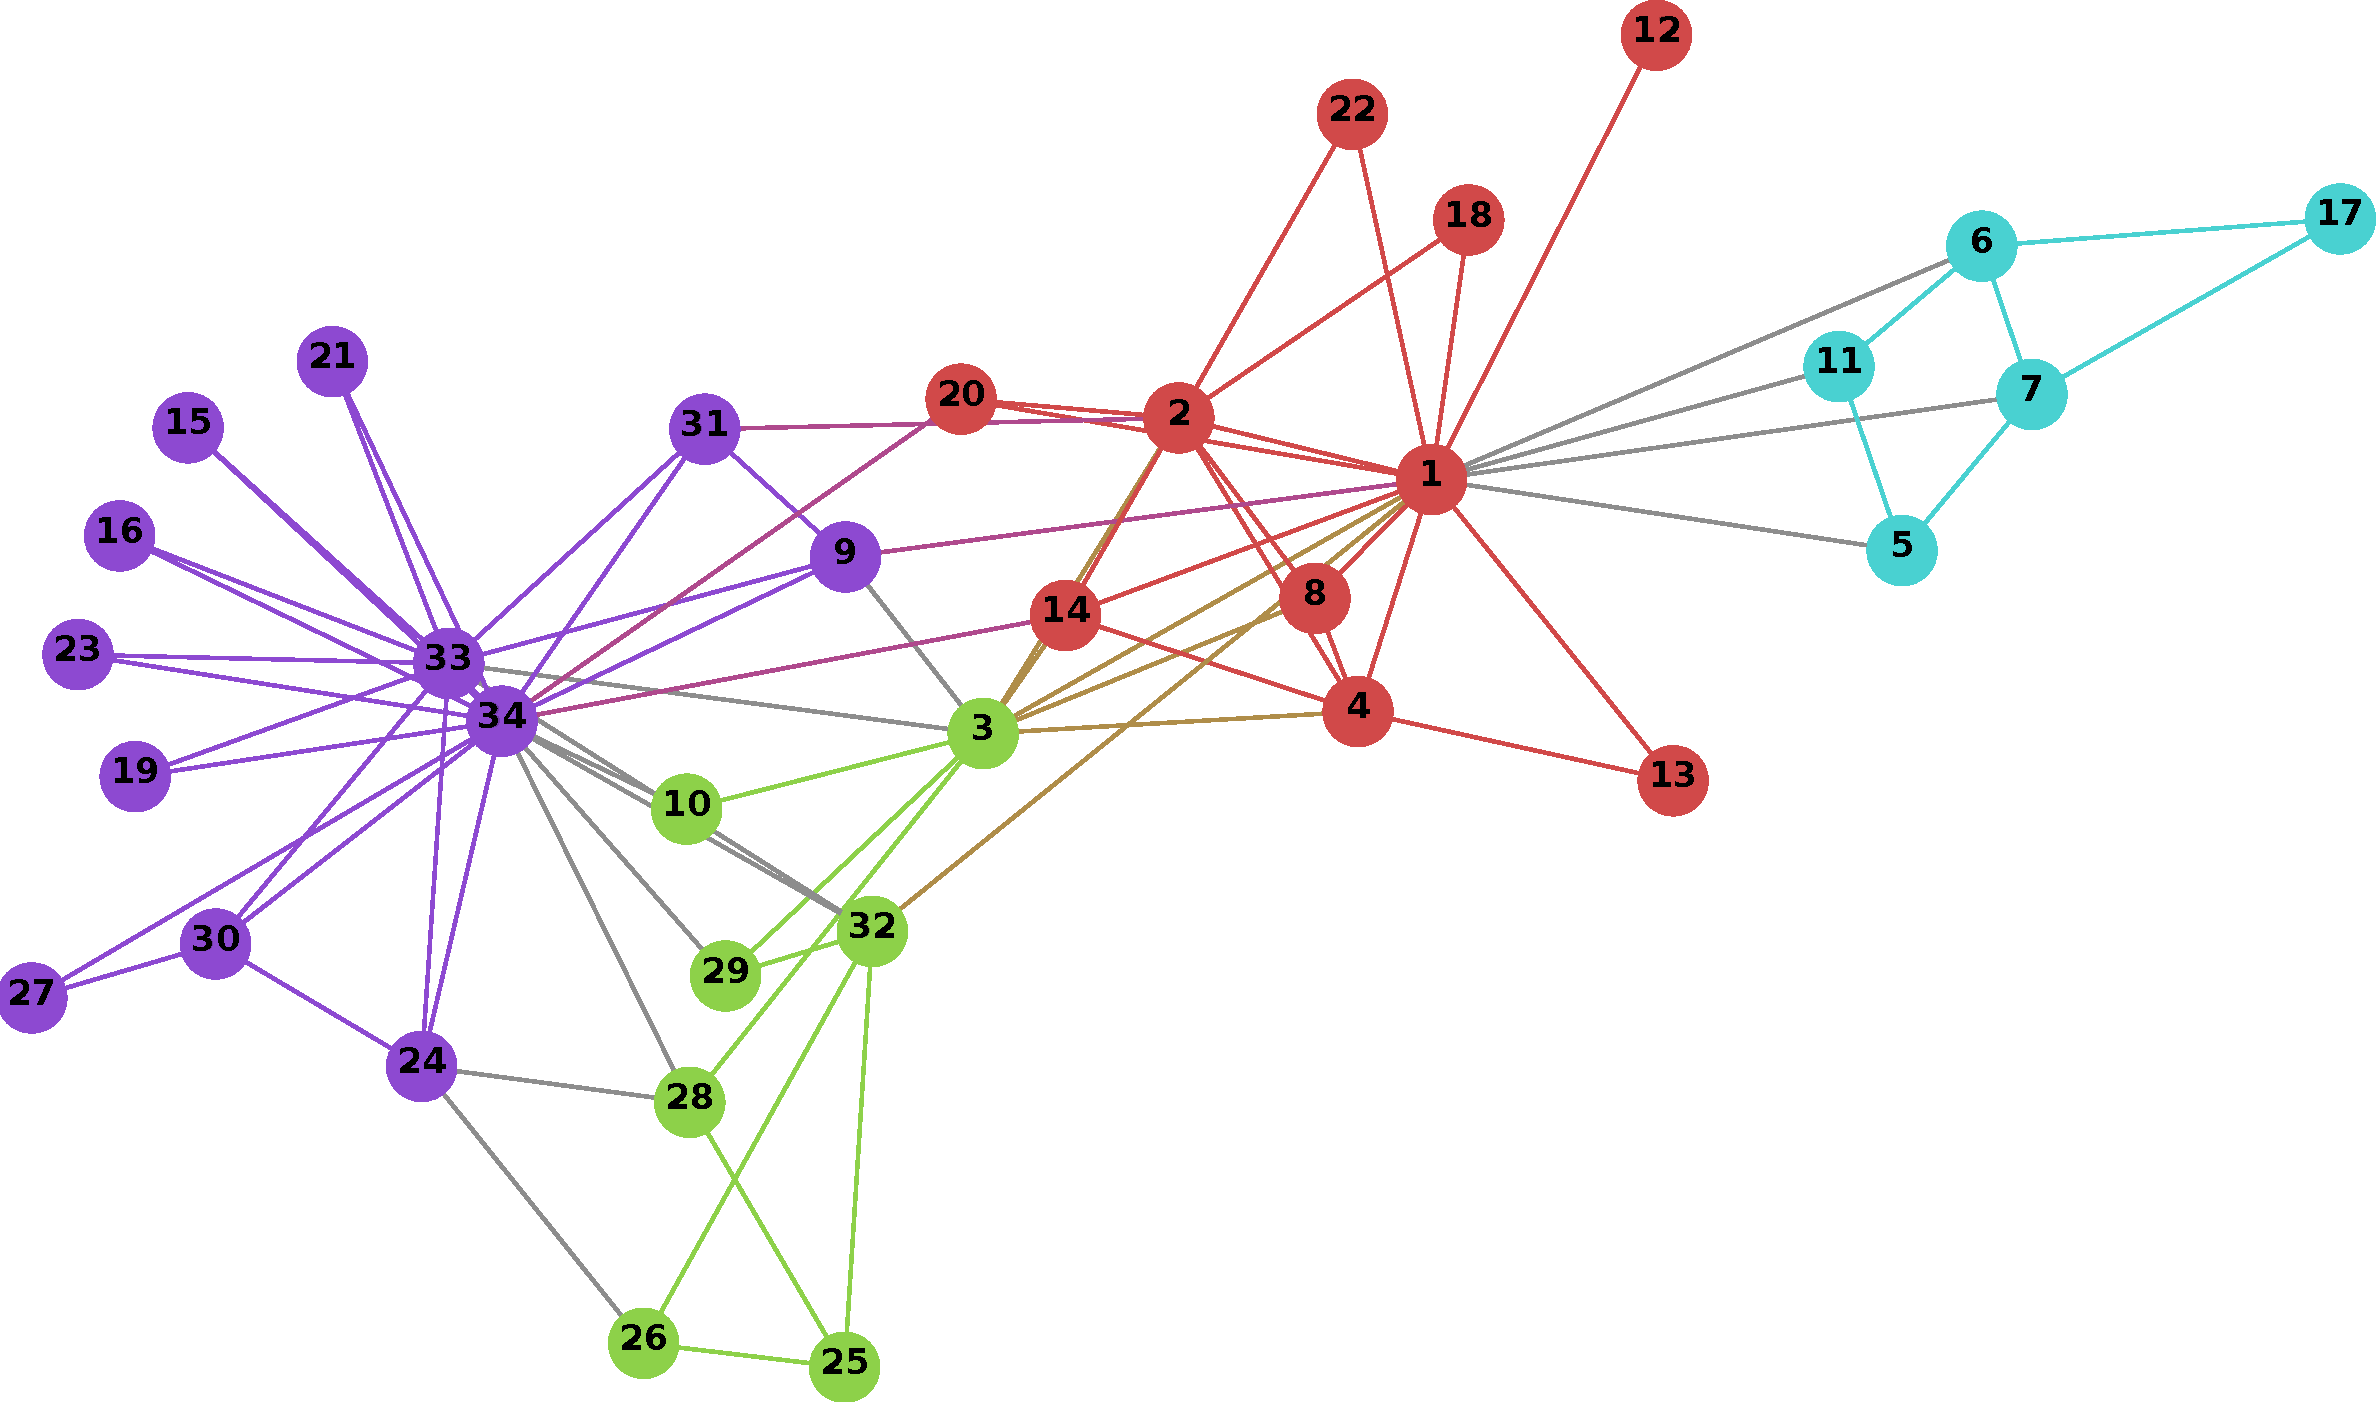
\includegraphics[width=\columnwidth]{figures/karate_graph.pdf}
                \caption{Input: Karate Graph}
                \label{fig:toy_example_graph}
        \end{subfigure}
        \begin{subfigure}[b]{0.48\columnwidth}
                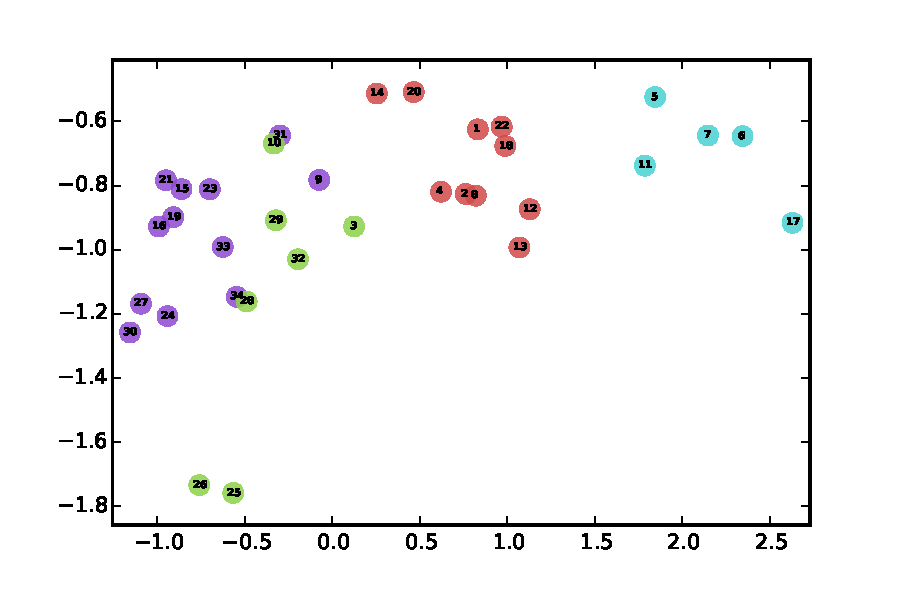
\includegraphics[width=\columnwidth]{figures/karate.pdf}
                \caption{Output: Representation}
                \label{fig:toy_example_embedding}
        \end{subfigure}
        \caption{Our proposed method \emph{learns} a latent space representation of social interactions in $\mathbb{R}^d$.  The learned representation encodes community structure so it can be easily exploited by standard classification methods. Here, our method is used on Zachary's Karate network \cite{zachary1977information} to generate a latent representation in $\mathbb{R}^2$.  
		Note the correspondence between community structure in the input graph and the embedding. Vertex colors represent a modularity-based clustering of the input graph.
		%To illustrate how community structure could be encoded, we color the vertices by cuts found through maximizing modularity in the original graph.
        %Interestingly, the embeddings encode community structure %found through maximizing modularity (vertex colors)
        %Community structure found by maximizing modularity (vertex colors) is preserved in the embedding.  
        %See Sections \ref{sec:method} for a description of our method, and Section \ref{sec:experiments} for results.
        }
        \label{fig:toy_example}
\end{figure}

\ouralgorithm\ takes a graph as input and produces a latent representation as an output.
The result of applying our method to the well-studied Karate network is shown in Figure \ref{fig:toy_example}.  
The graph, as typically presented by force-directed layouts, is shown in Figure \ref{fig:toy_example_graph}.
Figure \ref{fig:toy_example_embedding} shows the output of our method with 2 latent dimensions.
Beyond the striking similarity, we note that linearly separable portions of (\ref{fig:toy_example_embedding}) correspond to clusters found through modularity maximization in the input graph (\ref{fig:toy_example_graph}) (shown as vertex colors).

To demonstrate \ouralgorithm's potential in real world scenarios, we evaluate its performance on challenging multi-label network classification problems in large heterogeneous graphs.
In the relational classification problem, the links between feature vectors violate the traditional \emph{i.i.d.} assumption.  
Techniques to address this problem typically use approximate inference techniques \cite{neville2000iterative,Pearl:1988:PRI:534975} to leverage the dependency information to improve classification results.
%The choice of the seed of labeled vertices influence the performance greatly.
We distance ourselves from these approaches by learning label-independent representations of the graph.
Our representation quality is not influenced by the choice of labeled vertices, so they can be shared among tasks.
%Our representations are acquired through an objective function that maximizes, sound social networks characteristics.


\ouralgorithm\ outperforms other latent representation methods for creating \emph{social dimensions} \cite{Tang:2009:RLV:1557019.1557109,Tang:2011:Leveraging}, especially when labeled nodes are scarce.
Strong performance with our representations is possible with very simple linear classifiers (e.g. logistic regression).
%Our superior performance occurs even when using only 
%We observe superior performance, even using only simple classifiers as logistic regression.
%This confirms the merit of our learned representations on their own.
Our representations are general, and can be combined with any classification method (including iterative inference methods).
\ouralgorithm\ achieves all of that while being an online algorithm that is trivially parallelizable.


%%In recent years, the size and scope of attributed networks has grown dramatically.  
%%Networks describing the relationships between friends (Facebook, Twitter, Google Plus), entities (Knowledge Graph), products (Amazon), movie viewers (YouTube), and more have become essential parts of the Internet experience.
%%Although plentiful, these real-world networks frequently contain incomplete information.  
%%This can occur for a variety of reasons that can range from the benign (a user who neglects to fill out their profile), to the malicious (a merchant who omits relevant product details to deliberately mislead potential clients).  
%%In many cases, there is an economic incentive for trying to predict hidden attributes of the nodes (e.g. a user's receptivity to an advertisement).

%%This task can be framed as the network classification, or \emph{relational learning} problem \cite{getoor2007introduction,sen2008collective}.  
%%In the relational classification problem, the links between feature vectors violate the traditional \emph{i.i.d.} assumption.  
%%Techniques to address this problem typically use approximate inference techniques to leverage the dependency information to improve classification results.
%These approximate inference techniques can fail to converge, and cascade misinformation.

%%Another approach to the problem is to develop \emph{social dimensions}\cite{Tang:2009:RLV:1557019.1557109} which encode the relationships expressed in the original graph  in a continuous space.
%%The best proposed method to date requires global information, and expensive spectral decomposition \cite{Tang:2011:Leveraging}.

%%In this work, we generalize recent advancements in language modeling and unsupervised feature learning  (or \emph{deep learning}) from sequences of words to graphs.
%%Our algorithm, \ouralgorithm, \emph{learns} latent representations which encodes social relations in a continuous vector space.
%%This representations are very useful for classification, especially when many labels are missing.
%%Our approach is, to the best of our knowledge, the first time that deep learning techniques have been adapted for use in network classification.  


Our contributions are as follows: 
%Our contributions In this work, we present \ouralgorithm, an online algorithm for learning social representation, briefly, our contributions are:

\begin{itemize}

\item We introduce deep learning as a tool to analyze graphs, to build robust representations that are suitable for statistical modeling. \ouralgorithm\ learns structural regularities present within short random walks.

\item We extensively evaluate our representations on multi-label classification tasks on several social networks.
We show significantly increased classification performance in the presence of label sparsity, getting improvements 5\%-10\% of Micro $F_1$, on the sparsest problems we consider.
In some cases, \ouralgorithm's representations can outperform its competitors even when given 60\% less training data.

\item We demonstrate the scalability of our algorithm by building representations of web-scale graphs, (such as YouTube) using a parallel implementation.
Moreover, we describe the minimal changes necessary to build a streaming version of our approach.

\end{itemize}

The rest of the paper is arranged as follows.  In Sections \ref{sec:problem} and \ref{sec:SRL}, we discuss the problem formulation of classification in data networks, and how it relates to our work.  In Section \ref{sec:method} we present \ouralgorithm, our approach for Social Representation Learning.  We outline ours experiments in Section \ref{sec:experimental_design}, and present their results in Section \ref{sec:experiments}.  We close with a discussion of related work in Section \ref{sec:related}, and our conclusions.


\section{Problem Definition}
\label{sec:problem}

We consider the problem of classifying members of a social network into one or more categories.  
More formally, let $G=(V, E)$, where $V$ are the members of the network, and $E$ be its edges, $E \subseteq (V \times V)$.
Given a partially labeled social network $G_L = (V,E,X,Y)$, with attributes $X \in \mathbb{R}^{|V|\times S}$ where $S$ is the size of the feature space for each attribute vector, and $Y \in \mathbb{R}^{|V|\times |\mathcal{Y}|}$, $\mathcal{Y}$ is the set of labels.

In a traditional machine learning classification setting, we aim to learn a hypothesis $H$ that maps elements of $X$ to the labels set $\mathcal{Y}$.
In our case, we can utilize the significant information about the dependence of the examples embedded in the structure of $G$ to achieve superior performance.
%In fact, it not uncommon to have the network structure $E$ as the only information available to the classifier in the absence of node attributes $X$.
%Many real world graphs have been shown to have network structure which correlations with an output variable (known as \emph{homophily} \cite{mcpherson2001birds}, or positive relational autocorrelation \cite{getoor2007introduction}).

In the literature, this is known as the relational classification (or the \emph{collective classification} problem \cite{sen2008collective}).
Traditional approaches to relational classification pose the problem as an inference in an undirected Markov network, and then use iterative approximate inference algorithms (such as the iterative classification algorithm \cite{neville2000iterative}, Gibbs Sampling \cite{geman1984stochastic}, or label relaxation \cite{hummel1983foundations}) to compute the posterior distribution of labels given the network structure.

We propose a different approach to capture the network topology information.
Instead of mixing the label space as part of the feature space, we propose an unsupervised method which learns features that capture the graph structure \emph{independent} of the labels' distribution.

This separation between the structural representation and the labeling task avoids cascading errors, which can occur in iterative methods \cite{neville2008bias}.
Moreover, the same representation can be used for multiple classification problems concerning that network.
%, allowing modular learning and statistical strength to be shared across tasks.

Our goal is to learn $X_E \in \mathbb{R}^{|V|\times d}$, where $d$ is small number of latent dimensions.
%These latent representations are continuous real valued vectors.
These low-dimensional representations are distributed; meaning each social phenomena is expressed by a subset of the dimensions and each dimension contributes to a subset of the social concepts expressed by the space.

Using these structural features, we will augment the attributes space to help the classification decision.  
These features are general, and can be used with any classification algorithm (including iterative methods).  
However, we believe that the greatest utility of these features is their easy integration with simple machine learning algorithms. They scale appropriately in real-world networks, as we will show in Section \ref{sec:experiments}.


%\subsection{Assumptions}

%As we assume that the number of labeled examples are small fraction of the size of the network, we utilize the structure of the network to build socially justifiable representations with unsupervised algorithm.
%These representations will be dense real valued vectors $\in \mathbb{R}^d$  where $d$ in order of hundreds of dimensions.
%We will show that despite that representation learning is not influenced by the classes distribution that they are significantly helpful in capturing the network social topology.

%We aim to produce representations of the network nodes that correlates with node labels.

%Additionally, we assume: 

%each vertex may have additional attributes

%We also assume that the graph we are given should not be modified.

%We do not add edges.



\section{Learning Social Representations}
\label{sec:SRL}

%We view learning social representations as learning mappings between discrete space composed of the graphs nodes to a continuous space with lower dimensions.

We seek learning social representations with the following characteristics:
\begin{itemize}
\item \textbf{Adaptability} - Real social networks are constantly evolving;  new social relations should not require repeating the learning process all over again.


\item \textbf{Community aware} - The distance between latent dimensions should represent a metric for evaluating social similarity between the corresponding members of the network.
This allows generalization in networks with homophily.


%afford generalization, the representations proximity of members of the network should reflect the communities they belong to and the relations among these communities.
%Our learned representations should cluster in the space in several hierarchical levels depending on their membership to their communities.

% 3- Generalizable (encode big and small partitions)

\item \textbf{Low dimensional} - When labeled data is scarce, low-dimensional models generalize better, and speed up convergence and inference.
%We aim to learn representations with sufficient capacity to model the network structure, however, given the scarcity of labeled data, we prefer the smallest possible number of dimensions for modeling to avoid over-fitting and variance in results.
%This helps us to avoid the curse of dimensionality, generalize better, and speeds up convergence and inference.

\item \textbf{Continuous} - 
%Given that most of the typical classification models have a smooth decision boundaries, we prefer continuous space to represent our data to make learning more robust.
We require latent representations to model partial community membership in continuous space.
In addition to providing a nuanced view of community membership, a continuous representation has smooth decision boundaries between communities which allows more robust classification.

% 1- Low number of dimensions to make learning feasible

%We demand that our latent representations evolve along with them, and not require recomputation.
% this is amazing, put this part somewhere
%by requiring that updates in sublinear time.
%by requiring only \emph{local} information around a vertex to ...
%supports \emph{local updates}, ... the capability to 

%Given the growing size of social networks, we prefer an online learning procedure that produces useful intermediate representations that are immediately applicable.
%The online aspect give us the advantage of tracking the evolving nature of the network without starting over.
\end{itemize}

Our method for satisfying these requirements learns representation for vertices from a stream of short random walks, using optimization techniques originally designed for language modeling.
Here, we review the basics of both random walks and language modeling, and describe how their combination satisfies our requirements.

\subsection{Random Walks}
We denote a random walk rooted at vertex $v_i$ as $\mathcal{W}_{v_i}$.  
It is a stochastic process with random variables $\mathcal{W}^1_{v_i},\mathcal{W}^2_{v_i},\dots{},\mathcal{W}^k_{v_i}$ such that $\mathcal{W}^{k+1}_{v_i}$ is a vertex chosen at random from the neighbors of vertex $v_k$.
%A random walk of length $k$ on a possibly infinite graph $G$ with a root \textbf{0} is a stochastic process with random variables $X_{1},X_{2},\dots ,X_{k}$ such that$ X_{1}=0$ and ${X_{{i+1}}}$ is a vertex chosen uniformly at random from the neighbors of $X_{i}$.
Random walks have been used as a similarity measure for a variety of problems in content recommendation \cite{fouss2007random} and community detection \cite{andersen2006local}.
They are also the foundation of a class of \emph{output sensitive} algorithms which use them to compute local community structure information in time sublinear to the size of the input graph \cite{spielman2004nearly}.

It is this connection to local structure that motivates us to use a \emph{stream} of short random walks as our basic tool for extracting information from a network.
%then, might not only encode the local structure of the network but the evolving global topology.
%Typical methods like Laplacian, modularity sacrifice the local information and has resolution issues in their pursuit of capturing the global topology.
%Not to mention, the expensive computation requirement in terms of time and space.
In addition to capturing community information, using random walks as the basis for our algorithm gives us two other desirable properties.  First, 
%the information acquired from short random walks implicitly encodes local community information.
local exploration is easy to parallelize.  Several random walkers (in different threads, processes, or machines) can simultaneously explore different parts of the same graph.
Secondly, relying on information obtained from short random walks make it possible to accommodate small changes in the graph structure without the need for global recomputation.
We can iteratively update the learned model with new random walks from the changed region in time sub-linear to the entire graph.

%Designing the algorithm to use the random walks information, allows the representations to be aware of local structure such as communities.
%Moreover, the cheap cost of generating random walks, makes it easy to make the representations accommodate to any changes in the graph by feeding the learned model new random walks from the changed parts.


\subsection{Connection: Power laws}
Having chosen online random walks as our primitive for capturing graph structure, we now need a suitable method to capture this information.  
If the degree distribution of a connected graph follows a power law (is \emph{scale-free}), we observe that the frequency which vertices appear in the short random walks will also follow a power-law distribution.  

Word frequency in natural language follows a similar distribution, and techniques from language modeling account for this distributional behavior.
To emphasize this similarity we show two different power-law distributions in Figure \ref{fig:power_law}. 
The first comes from a series of short random walks on a scale-free graph, and the second comes from the text of 100,000 articles from the English Wikipedia.

A core contribution of our work is the idea that techniques which have been used to model natural language (where the symbol frequency follows a power law distribution (or \emph{Zipf's law})) can be re-purposed to model community structure in networks.
\begin{figure}
	\centering
      \begin{subfigure}[b]{0.48\columnwidth}
                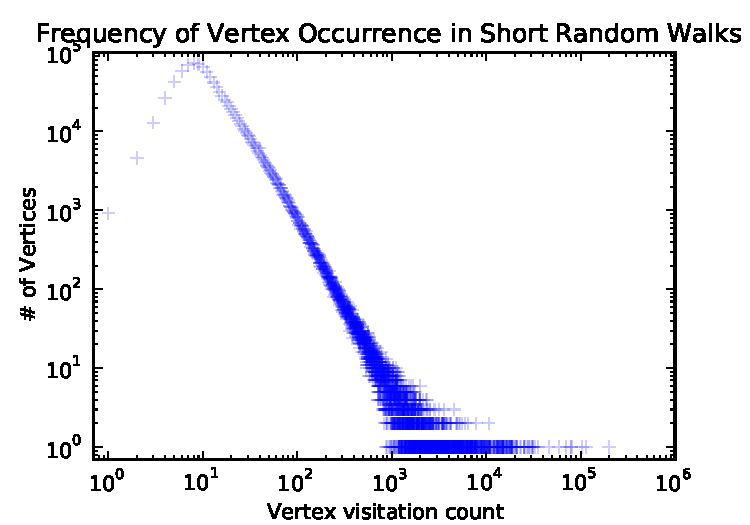
\includegraphics[width=\columnwidth]{figures/powerlaw/youtube-powerlaw}
		\caption{YouTube Social Graph}
		\label{fig:powerlaw-youtube}
	\end{subfigure}
      \begin{subfigure}[b]{0.48\columnwidth}
                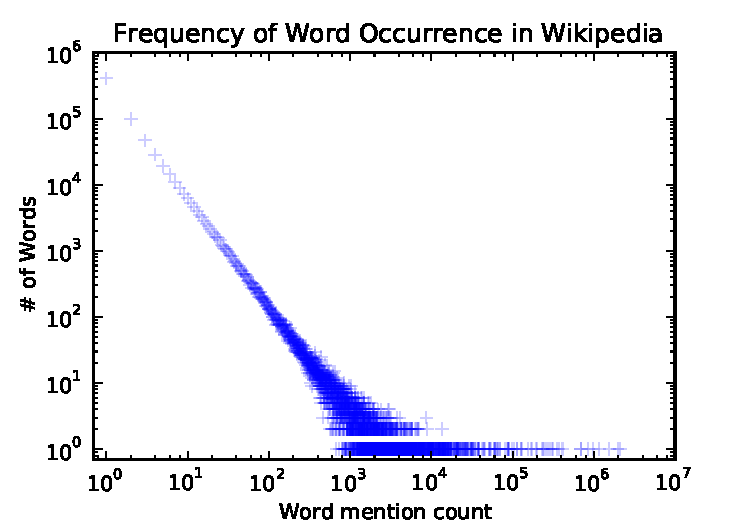
\includegraphics[width=\columnwidth]{figures/powerlaw/wiki-powerlaw}	
		\caption{Wikipedia Article Text}
		\label{fig:powerlaw-wiki}
	\end{subfigure}
\caption{The power-law distribution of vertices appearing in short random walks (\ref{fig:powerlaw-youtube}) follows a power-law, much like the distribution of words in natural language (\ref{fig:powerlaw-wiki}).  
%We propose using techniques from language modeling to learn better vertex representations.
}
\label{fig:power_law}
\end{figure}
We spend the rest of this section reviewing the growing work in language modeling, and transforming it to learn representations of vertices which satisfy our criteria.

%To satisfy the rest of our criteria, we turn our attention to the growing work in language modeling and using an interesting connection between the two problems.


\subsection{Language Modeling}
%The distribution of words in natural language has been shown to follow a power law\cite{}, as has the degree distribution in many real world graphs\cite{}.
%To emphasize this point we present three different exponential distributions in Figure \ref{fig:power_law}. The degree distribution of a connected graph, the frequency with which a node appears in a number of short random walks, and the word frequency in a selection of text from the English Wikipedia.
The goal of language modeling is estimate the likelihood of a specific sequence of words appearing in a corpus.
More formally, given a sequence of words $$W_{1}^{n} = (w_0, w_1, \cdots, w_n)$$ where $w_i \in \mathcal{V}$ ($\mathcal{V}$ is the vocabulary), we would like to maximize the $\Pr(w_n| w_0, w_1, \cdots, w_{n-1})$ over all the training corpus.
\comment{
The performance of the model will be evaluated on held out testing corpus using a perplexity score $PP$ as defined below
\begin{equation}
PP = \frac{1}{\sqrt[n]{P(W_1^n)}}
\end{equation}}

Recent work in representation learning has focused on using probabilistic neural networks to build general representations of words which extend the scope of language modeling beyond its original goals.

In this work, we present a generalization of language modeling to explore the graph through a stream of short random walks.
These walks can be thought of short sentences and phrases in a special language.
The direct analog is to estimate the likelihood of observing vertex $v_i$ given all the previous vertices visited so far in the random walk.

$$\Pr\big(v_{i}\mid( v_1, v_2, \cdots, v_{i-1})\big)$$

Our goal is to learn a latent representation, not only a probability distribution of node co-occurrences, and so we introduce a mapping function $\Phi \colon v \in V \mapsto \mathbb{R}^{|V|\times d}$.
This mapping $\Phi$ represents the latent social representation associated with each vertex $v$ in the graph.
(In practice, we represent $\Phi$ by a $|V| \times d$ matrix of free parameters, which will serve later on as our $X_E$.)
The problem then, is to estimate the likelihood:

\begin{equation}
\Pr\Big(v_i \mid \big(\Phi(v_1), \Phi(v_2), \cdots, \Phi(v_{i-1})\big)\Big)
\end{equation}


% 2 Why this won't work
However as the walk length grows, computing this objective function becomes unfeasible.

% 3 A solution:  Mikolov
A recent relaxation in language modeling \cite{word2vec1,word2vec2} turns the prediction problem on its head.
First, instead of using the context to predict a missing word, it uses one word to predict the context.
Secondly, the context is composed of the words appearing to right side of the given word as well as the left side.
Finally, it removes the ordering constraint on the problem.
Instead, the model is required to maximize the probability of any word appearing in the context without the knowledge of its offset from the given word.


In terms of vertex representation modeling, this yields the optimization problem:


\begin{equation}
\begin{aligned}
& \underset{\Phi}{\text{minimize}}
& & -\log \Pr\big(\{v_{i-w}, \cdots, v_{i-1}, v_{i+1}, \cdots, v_{i+w}\}\mid \Phi(v_i) \big) \\
\end{aligned}
\label{eq:objective}
\end{equation}

%Notice, that the objective function models the transition probability of random walks of length $2w$.
We find these relaxations are particularly desirable for social representation learning.
First, the order independence assumption better captures a sense of `nearness' that is provided by random walks.
%The neighborhood of a vertex does not follow a partial order relation.
%Hence, the order independence assumption is appropriate.
Moreover, this relaxation is quite useful for speeding up the training time by building small models as one vertex is given at a time.

Solving the optimization problem from Eq. \ref{eq:objective} builds representations that capture the shared similarities in local graph structure between vertices.
Vertices which have similar neighborhoods will acquire similar representations (encoding co-citation similarity), and allowing generalization on machine learning tasks.


By combining both truncated random walks and neural language models we formulate a method which satisfies all of our desired properties.
This method generates representations of social networks that are low-dimensional, and exist in a continuous vector space.
Its representations encode latent forms of community membership, and because the method outputs useful intermediate representations, it can adapt to changing network topology.




%\begin{equation*}
%\sum_{t=1}^{T} \Big[\sum_{j=-l}^{l} \log p(v_{t+j}|v_t)\Big]
%\end{equation*}


%These techniques well known ideas use distributed word representations ideas developed by Hinton in the 1980s to 



%Language modeling goal is to model the patterns of language usage learned from a corpus to predict the future 
% Random walk

% Community preserving technique (Pastor of the village)

% We do not require full information about
% full connectivity of the network or any of its verices.
% - Network topology
% - Vertex neighborhood
% - full path between two nodes

% The closest format to the data available to our algorithm is language sentences, we look into language modeling to extract representation from such partial information.
% Our target is not to build a language model, so we use the ones that develop representation through the modeling process


%What should a social representation do?

% 2- Random walk is amazing to capture the neighborhood.
% 1- Nodes structural-similar iff have similar neighborhood. (loosely defined)
% 4- Similar nodes should have close representations.
% 5- Orthogonal information to the attributes and labels.  (it should add information to the system)
% 6- interpretability?
% What characteristics should it have?



% Talk about Random walks as a way to characterize

% We approach 

% What is the intuition behind our approach

%Social networks are free scale networks, where degree frequency distributions is a power law distribution.
%Such distribution is observed in word frequency distribution.
%We hypothesize that the algorithms that are built to symbolic data as language vocabulary are able to play the same role 
%As the distribution of word frequency is a power law distribution, a similar 

\section{Method}
\label{sec:method}

\begin{figure*}

\begin{subfigure}[b]{0.30\textwidth}
\adjustbox{trim={0.0\width} {.0\height} {0.7\width} {.05\height},clip}{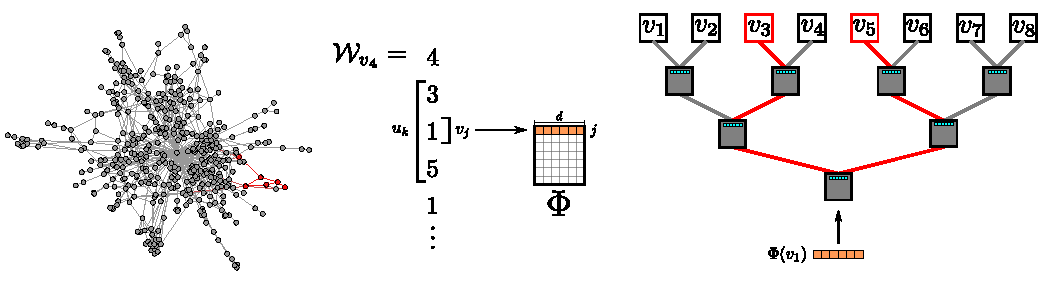
\includegraphics{figures/deepwalk_overview}}
\caption{Random walk generation.}
\label{fig:graph}
\end{subfigure}
\begin{subfigure}[b]{0.30\textwidth}
\adjustbox{trim={.3\width} {.15\height} {0.4\width} {.05\height},clip}{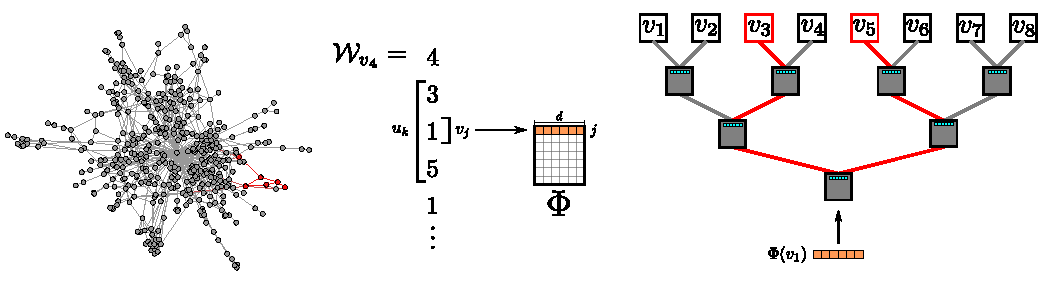
\includegraphics{figures/deepwalk_overview}}
\caption{Representation mapping.}
\label{fig:phi}
\end{subfigure}
\begin{subfigure}[b]{0.4\textwidth}
\adjustbox{trim={.605\width} {.1\height} {0.0\width} {.04\height},clip}{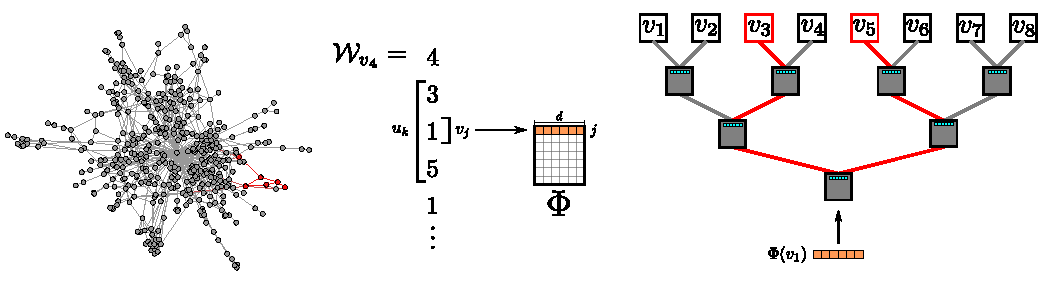
\includegraphics{figures/deepwalk_overview}}
\caption{Hierarchical Softmax.}
\label{fig:hsm}
\end{subfigure}

\caption{Overview of \ouralgorithm.
We slide a window of length $2w+1$ over the random walk $\mathcal{W}_{v_4}$, mapping the central vertex $v_1$ to its representation $\Phi(v_1)$.
Hierarchical Softmax factors  out $\Pr(v_3 \mid \Phi(v_1))$ and $\Pr(v_5 \mid \Phi(v_1))$ over sequences of probability distributions corresponding to the paths starting at the root and ending at $v_3$ and $v_5$.
The representation $\Phi$ is updated to maximize the probability of $v_1$ co-occurring with its context $\{v_3, v_5\}$.
}
\end{figure*}

In this section we discuss the main components of our algorithm. 
%Next we analyze the computational complexity and parallelizablity of \ouralgorithm.
We also present several variants of our approach and discuss their merits.

\subsection{Overview}
As in any language modeling algorithm, the only required input is a corpus and a vocabulary $\mathcal{V}$.
\ouralgorithm\  considers a set of short truncated random walks its own corpus, and the graph vertices as its own vocabulary ($\mathcal{V} = V$).
While it is beneficial to know the $V$ and the frequency distribution of vertices in the random walks ahead of the training, it is not necessary for the algorithm to work as we will show in \ref{sec:hsm}.

\subsection{Algorithm: {\large \ouralgorithm}}
The algorithm consists of two main components; first a random walk generator and second an update procedure.

\begin{algorithm}[t]
\begin{algorithmic}[1]
\REQUIRE graph $G(V,E)$\\ window size $w$\\ embedding size $d$\\ walks per vertex $\mathcal{\gamma}$ \\ walk length $t$
\ENSURE matrix of vertex representations $\Phi \in \mathbb{R}^{|V| \times d}$
	\STATE Initialization: Sample $\Phi$ from $\mathcal{U}^{|V| \times d}$
	\STATE Build a binary Tree $T$ from $V$
	\FOR{$i=0$ to $\mathcal{\gamma}$}
		\STATE	$\mathcal{O} = \text{Shuffle}(V)$
        \FOR{\textbf{each} $v_i \in \mathcal{O}$}
		\STATE $\mathcal{W}_{v_i} = RandomWalk(G, v_i, $t$) $
		\STATE SkipGram($\Phi$, $\mathcal{W}_{v_i}$, $w$)
		 \ENDFOR
	\ENDFOR
\end{algorithmic}
\caption{\ouralgorithm($G$, $w$, $d$, $\gamma$, $t$)}
\label{alg:deepwalk}
\end{algorithm}

The random walk generator takes a graph $G$ and samples uniformly a random vertex $v_i$ as the root of the random walk $\mathcal{W}_{v_i}$.
A walk samples uniformly from the neighbors of the last vertex visited until the maximum length ($t$) is reached.
While we set the length of our random walks in the experiments to be fixed, there is no restriction for the random walks to be of the same length.
%Actually, we could start one walk per vertex and walk infinitely as long as we add restarts to the generator.
These walks could have restarts (i.e. a teleport probability of returning back to their root), but
our preliminary results did not show any advantage of using restarts.
In practice, our implementation specifies a number of random walks $\mathcal{\gamma}$ of length $t$ to start at each vertex.


Lines 3-9 in Algorithm \ref{alg:deepwalk} shows the core of our approach.
The outer loop specifies the number of times, $\mathcal{\gamma}$, which we should start random walks at each vertex.
We think of each iteration as making a `pass' over the data and sample one walk per node during this pass.
At the start of each pass we generate a random ordering to traverse the vertices.  
This is not strictly required, but is well-known to speed up the convergence of stochastic gradient descent.

In the inner loop, we iterate over all the vertices of the graph.  
For each vertex $v_i$ we generate a random walk $|\mathcal{W}_{v_i}| = t$, and then use it to update our representations (Line 7).
We use the SkipGram algorithm \cite{word2vec1} to update these representations in accordance with our objective function in Eq. \ref{eq:objective}.
%Our approach is flexible, as we can replace SkipGram with any other continuous space language model algorithm.


\subsubsection{SkipGram}
SkipGram is a language model that maximizes the co-occurrence probability among the words that appear within a window, $w$, in a sentence \cite{word2vec1}.
%In the context of random walks, we are approximating the random walk transition probability matrix $P^{w}$.

Algorithm \ref{alg:skipgram} iterates over all possible collocations in  random walk that appear within the window $w$ (lines 1-2).
For each, we map each vertex $v_j$ to its current representation vector $\Phi(v_j) \in \mathbb{R}^d$ (See Figure \ref{fig:phi}).
Given the representation of $v_j$, we would like to maximize the probability of its neighbors in the walk (line 3).
We can learn such posterior distribution using several choices of classifiers.
For example, modeling the previous problem using logistic regression would result in a huge number of labels  that is equal to $|V|$ which could be in millions or billions.
Such models require large amount of computational resources that could span a whole cluster of computers \cite{nnlm}.
To speed the training time, Hierarchical Softmax \cite{hsm1,hsm2} can be used to approximate the probability distribution.


\begin{algorithm}[t]
\begin{algorithmic}[1]
    \FOR{\textbf{each} $v_j \in \mathcal{W}_{v_i}$}
		\FOR{\textbf{each} $u_k \in \mathcal{W}_{v_i}[j-w: j+w]$}
				\STATE  $J(\Phi) = - \log{\Pr(u_k \mid \Phi(v_j))}$
	        	\STATE $\Phi = \Phi - \alpha * \frac{\partial J}{\partial \Phi}$
		\ENDFOR

	\ENDFOR

\end{algorithmic}
\caption{SkipGram($\Phi$, $\mathcal{W}_{v_i}$, $w$)}
\label{alg:skipgram}
\end{algorithm}


\subsubsection{Hierarchical Softmax}
\label{sec:hsm}
Given that $u_k \in V$, calculating $\Pr(u_k \mid \Phi(v_j))$ in line 3 is not feasible.
Computing the partition function (normalization factor) is expensive.
If we assign the vertices to the leaves of a binary tree, the prediction problem turns into maximizing the probability of a specific path in the tree (See Figure \ref{fig:hsm}).
If the path to vertex $u_k$ is identified by a sequence of tree nodes $(b_0, b_1, \dots, b_{\ceil{\log|V|}})$, ($b_0$ = root, $b_{\ceil{\log|V|}} = u_k$) then $$\Pr(u_k \mid \Phi(v_j)) = \prod_{l=1}^{\ceil{\log|V|}} \Pr(b_l \mid \Phi(v_j)) $$

Now, $\Pr(b_l \mid \Phi(v_j))$ could be modeled by a binary classifier that is assigned to the parent of the node $b_l$.
This reduces the computational complexity of calculating $\Pr(u_k \mid \Phi(v_j))$ from $O(|V|)$ to $O(\log |V|)$.

We can speed up the training process further, by assigning shorter paths to the frequent vertices in the random walks.
Huffman coding is used to reduce the access time of frequent elements in the tree.

\subsubsection{Optimization}
The model parameter set is $\{\Phi, T\}$ where the size of each is $O(d|V|)$.
Stochastic gradient descent (SGD) \cite{sgd} is used to optimize these parameters (Line 4, Algorithm \ref{alg:skipgram}).
The derivatives are estimated using the back-propagation algorithm.
The learning rate $\alpha$ for SGD is initially set to 2.5\% at the beginning of the training and then decreased linearly with the number of vertices that are seen so far.


\comment{
\subsection{Complexity}
\todo{I want to show performance vs L for blogcatalog, I want to say that we converge quickly, we can reduce the size of walks in future work.}

The total length of the walks is $L = \gamma t$, then complexity of our approach is $O(dwL\log |V|)$.
Figure \ref{} shows the relation between the quality of the embeddings and length of the walks seen so far in the training.
While our model build representations that are quite useful at early stages.
The complexity of the graph structure plays a main role in how much fast we can build a good estimate of the graph topology.
As the number of possible transitions in all our walks is bounded by the number of edges $m$, we can bound our complexity to be $O(dwm\log |V|)$.
The choice of $w$ in free scale networks is bounded by the network diameter, as there is decreasing amount of information in the collocations that span the whole graph.
As $w$ is bounded by  a constant, we can see that our complexity is $O(dm\log |V|)$
}

\subsection{Parallelizability}
As shown in Figure \ref{fig:power_law} the frequency distribution of vertices in random walks of social network and words in a language both follow a power law.
This results in a long tail of infrequent vertices, therefore, the updates that affect $\Phi$ will be sparse in nature.
This allows us to use asynchronous version of stochastic gradient descent (ASGD), in the multi-worker case.
Given that our updates are sparse and we do not acquire a lock to access the model shared parameters, ASGD will  achieve an optimal rate of convergence \cite{hogwild}.
While we run experiments on one machine using multiple threads, it has been demonstrated that this technique is highly scalable, and can be used in very large scale machine learning \cite{largedeep}.
%scaling up the training to a cluster of computers already demonstrated on large scale machine learning applications .
Figure \ref{fig:parallel} presents the effects of parallelizing \ouralgorithm.  It shows the speed up in processing \blogcatalog\ and \flickr\ networks is consistent as we increase the number of workers to 8 (Figure \ref{fig:parallel_speed}).
It also shows that there is no loss of predictive performance relative to the running \ouralgorithm\ serially (Figure \ref{fig:parallel_performance}).

%$n = |V|$

%$O(dn \log n)$, unless using negative sampling, $O(dn)$

%Normal SVD is $O(n^3)$

%Brand's fast SVD is $O(nmd)$ \cite{brand2003fast}, and supports .  Other approaches include using SGD to directly learn the SVD (like Simon Funk did for the netflicks prize) \cite{}.

\subsection{Algorithm Variants}
Here we discuss some variants of our proposed method, which we believe may be of interest.

\subsubsection{Streaming}
\label{variant_streaming}
One interesting variant of this method is a \emph{streaming} approach, which could be implemented without knowledge of the entire graph.
In this variant small walks from the graph are passed directly to the representation learning code, and the model is updated directly.
%Re-purposing the proposed algorithm in Section \ref{sec:method} to work in a streaming mode requires minimal effort.
%Whenever a new random walk is received, simply pass it to the language model directly.
%In such a streaming environment, there is no need to have access to the graph anymore.
Some modifications to the learning process will also be necessary.
First, using a decaying learning rate will no longer be possible.  Instead, we can initialize the learning rate $\alpha$ to a small constant value.  
This will take longer to learn, but may be worth it in some applications.
Second, we cannot necessarily build a tree of parameters any more.
If the cardinality of $V$ is known (or can be bounded), we can build the Hierarchical Softmax tree for that maximum value. 
Vertices can be assigned to one of the remaining leaves when they are first seen.
If we have the ability to estimate the vertex frequency a priori, we can also still use Huffman coding to decrease frequent element access times.

\subsubsection{Non-random walks}
%Another interesting variant comes from the way that graphs are created in the real world.
%In many real world graphs (click graphs, etc), the graph is built by \emph{non-random} walks made by users interacting with a system.  
Some graphs are created as a by-product of agents interacting with a sequence of elements (e.g. users' navigation of pages on a website).  
When a graph is created by such a stream of \emph{non-random} walks, we can use this process to feed the modeling phase directly.
Graphs sampled in this way will not only capture information related to network structure, but also to the frequency at which paths are traversed.

In our view, this variant also encompasses language modeling. Sentences can be viewed as purposed walks through an appropriately designed language network, and 
language models like SkipGram are designed to capture this behavior.

This approach can be combined with the streaming variant (Section \ref{variant_streaming}) to train features on a continually evolving network without ever explicitly constructing the entire graph.  
Maintaining representations with this technique could enable web-scale classification without the hassles of dealing with a web-scale graph.

\begin{figure}[t!]
\centering
\begin{subfigure}[b]{0.5\columnwidth}	
\centering
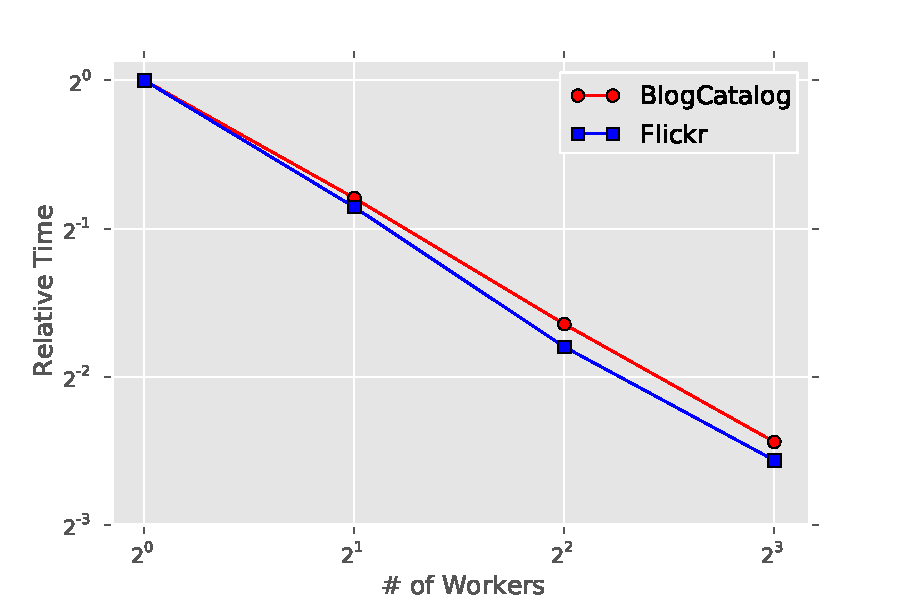
\includegraphics[width=\columnwidth]{figures/scalability_time.pdf}
\caption{Running Time}
\label{fig:parallel_speed}
\end{subfigure}%
\begin{subfigure}[b]{0.5\columnwidth}	
\centering
 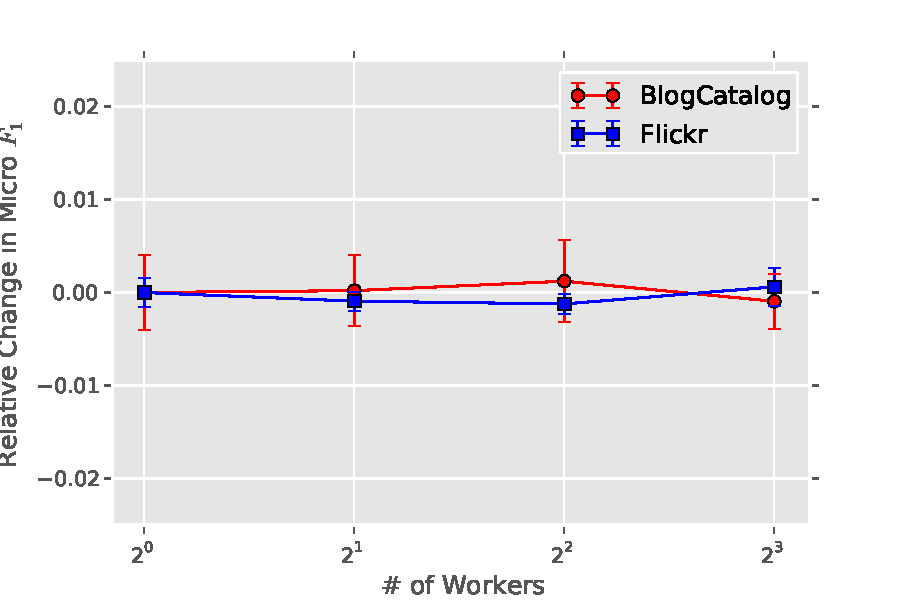
\includegraphics[width=\columnwidth]{figures/scalability_perf.pdf}
\caption{Performance} 
\label{fig:parallel_performance}
\end{subfigure}
\caption{Effects of parallelizing \ouralgorithm}
\label{fig:parallel}
\end{figure}


\begin{table}[t!]
\begin{center}
  \begin{tabular}{ c | c | c | c }
	Name & \blogcatalog & \flickr & \youtube \\
    \hline
	$|V|$ & 10,312 & 80,513 & 1,138,499 \\
	$|E|$ & 333,983 & 5,899,882 & 2,990,443 \\
	$|\mathcal{Y}|$ & 39 & 195 & 47 \\
	Labels & Interests & Groups & Groups \\

%  \cora & Citation & 2,708 & 5,429 & 7 & Document Categories & Bag-of-Words\\
%  \citeseer & Citation & 3,312 & 4,732 & 6& Document Categories & Bag-of-Words\\
%  \hline
  \end{tabular}
  \caption{Graphs used in our experiments.}
  \label{table.graph_info}  
\end{center}
\end{table}


\section{Experimental Design}
\label{sec:experimental_design}

In this section we provide an overview of the datasets and methods which we will use in our experiments.  Code and data to reproduce our results will be available at the first author's website.

\subsection{Datasets}

An overview of the graphs we consider in our experiments is given in Figure \ref{table.graph_info}.

\begin{itemize}[itemsep=1pt, topsep=5pt, partopsep=0pt]
%\item \cora\text{} and \citeseer \cite{sen2008collective} are directed networks of citations between academic research papers.  Labels correspond to the field of research of each paper, and the networks have binary features which represent whether a particular word appeared in the paper's abstracts or not.  We transform these networks to undirected ones for our analysis.
\item \blogcatalog \cite{Tang:2009:RLV:1557019.1557109} is a network of social relationships provided by blogger authors.  The labels represent the topic categories provided by the authors.
\item \flickr \cite{Tang:2009:RLV:1557019.1557109} is a network of the contacts between users of the photo sharing website.  The labels represent the interest groups of the users such as `\emph{black and white photos}'.
\item \youtube \cite{tang2009scalable} is a social network between users of the popular video sharing website.  The labels here represent groups of viewers that enjoy common video genres (e.g. \emph{anime} and \emph{wrestling}).
\end{itemize}

\subsection{Baseline Methods}
To validate the performance of our approach we compare it against a number of baselines:

\begin{itemize}[itemsep=0pt, topsep=5pt, partopsep=0pt]
\item \socdimL \cite{Tang:2011:Leveraging}: This method generates a representation in $\mathbb{R}^d$ from the $d$-smallest eigenvectors of $\Laplacian$, the normalized graph Laplacian of $G$.  
Utilizing the eigenvectors of $\Laplacian$ implicitly assumes that graph cuts will be useful for classification.

\item \socdimB \cite{Tang:2009:RLV:1557019.1557109}: This method generates a representation in $\mathbb{R}^d$ from the top-$d$ eigenvectors of $B$, the Modularity matrix of $G$.  
The eigenvectors of $B$ encode information about modular graph partitions of $G$\cite{newman2006modularity}. Using them as features assumes that modular graph partitions will be useful for classification.

\item \socdimA \cite{tang2009scalable}: This method uses $k$-means clustering to cluster the adjacency matrix of $G$.  Its has been shown to perform comparably to the \socdimB\text{} method, with the added advantage of scaling to graphs which are too large for spectral decomposition.

\item wvRN\cite{Macskassy03asimple}: The weighted-vote Relational Neighbor is a relational classifier.
Given the neighborhood $\mathcal{N}_i$ of vertex $v_i$, wvRN estimates $\Pr(y_i|\mathcal{N}_i)$  with the (appropriately normalized) weighted mean of its neighbors (i.e $\Pr(y_i|\mathcal{N}_i) = \frac{1}{Z}\sum_{v_j \in \mathcal{N}_i}{w_{ij}\Pr(y_j \mid \mathcal{N}_j)}$).
It has shown surprisingly good performance in real networks, and has been advocated as a sensible relational classification baseline \cite{macskassy2007classification}.

\item Majority:  This na\"{\i}ve method simply chooses the most frequent labels in the training set.
\end{itemize}

\section{Experiments}
\label{sec:experiments}

\begin{table*}[p]
\begin{center}

\begin{tabular}{l|l|r|r|r|r|r|r|r|r|r}
 & \% Labeled Nodes & 10\% & 20\% & 30\% & 40\% & 50\% & 60\% & 70\% & 80\% & 90\% \\ \hline
  & & & & & & & & & & \\ 
  \rowcolor{high}
 & \ouralgorithm & \textbf{36.00} & \textbf{38.20} & \textbf{39.60} & \textbf{40.30} & 
 \textbf{41.00} & \textbf{41.30} & 41.50 & 41.50 & 42.00 \\
 & \socdimL & 31.06 & 34.95 & 37.27 & 38.93 & 39.97 & 40.99 & \textbf{41.66} & \textbf{42.42} & \textbf{42.62} \\
 & \socdimA & 27.94 & 30.76 & 31.85 & 32.99 & 34.12 & 35.00 & 34.63 & 35.99 & 36.29 \\
Micro-F1(\%) & \socdimB & 27.35 & 30.74 & 31.77 & 32.97 & 34.09 & 36.13 & 36.08 & 37.23 & 38.18 \\
 & wvRN & 19.51 & 24.34 & 25.62 & 28.82 & 30.37 & 31.81 & 32.19 & 33.33 & 34.28 \\
 & Majority & 16.51 & 16.66 & 16.61 & 16.70 & 16.91 & 16.99 & 16.92 & 16.49 & 17.26 \\
 & & & & & & & & & & \\ \hline
 & & & & & & & & & & \\
 \rowcolor{high} 
 & \ouralgorithm & \textbf{21.30} & \textbf{23.80} & 25.30 & 26.30 & 27.30 & 27.60 & 27.90 & 28.20 & 28.90 \\ 
 & \socdimL & 19.14 & 23.57 & \textbf{25.97} & \textbf{27.46} & \textbf{28.31} & \textbf{29.46} & \textbf{30.13} & \textbf{31.38} & \textbf{31.78} \\
 & \socdimA & 16.16 & 19.16 & 20.48 & 22.00 & 23.00 & 23.64 & 23.82 & 24.61 & 24.92 \\
Macro-F1(\%) & \socdimB & 17.36 & 20.00 & 20.80 & 21.85 & 22.65 & 23.41 & 23.89 & 24.20 & 24.97 \\
 & wvRN & 6.25 & 10.13 & 11.64 & 14.24 & 15.86 & 17.18 & 17.98 & 18.86 & 19.57 \\ 
 & Majority & 2.52 & 2.55 & 2.52 & 2.58 & 2.58 & 2.63 & 2.61 & 2.48 & 2.62 \\
\end{tabular}
\end{center}
\caption{Multi-label classification results in \blogcatalog}
\label{tbl:blogcatalog}
\end{table*}


\begin{table*}[p]
\begin{center}
\begin{tabular}{l|l|r|r|r|r|r|r|r|r|r|r}
 & \% Labeled Nodes & 1\% & 2\% & 3\% & 4\% & 5\% & 6\% & 7\% & 8\% & 9\% & 10\% \\ \hline
 & & & & & & & & & & & \\
 \rowcolor{high} 
 & \ouralgorithm & \textbf{32.4} & \textbf{34.6} & \textbf{35.9} & \textbf{36.7} & \textbf{37.2} & \textbf{37.7} & \textbf{38.1} & \textbf{38.3} & \textbf{38.5} & \textbf{38.7} \\
 & \socdimL & 27.43 & 30.11 & 31.63 & 32.69 & 33.31 & 33.95 & 34.46 & 34.81 & 35.14 & 35.41 \\
Micro-F1(\%) & \socdimA & 25.75 & 28.53 & 29.14 & 30.31 & 30.85 & 31.53 & 31.75 & 31.76 & 32.19 & 32.84 \\
 & \socdimB & 22.75 & 25.29 & 27.3 & 27.6 & 28.05 & 29.33 & 29.43 & 28.89 & 29.17 & 29.2 \\
 & wvRN & 17.7 & 14.43 & 15.72 & 20.97 & 19.83 & 19.42 & 19.22 & 21.25 & 22.51 & 22.73 \\
 & Majority & 16.34 & 16.31 & 16.34 & 16.46 & 16.65 & 16.44 & 16.38 & 16.62 & 16.67 & 16.71 \\
 & & & & & & & & & & & \\ \hline
 & & & & & & & & & & & \\
 \rowcolor{high}
 & \ouralgorithm & \textbf{14.0} & 17.3 & \textbf{19.6} & \textbf{21.1} & \textbf{22.1} & \textbf{22.9} & \textbf{23.6} & \textbf{24.1} & \textbf{24.6} & \textbf{25.0} \\
 & \socdimL & 13.84 & \textbf{17.49} & 19.44 & 20.75 & 21.60 & 22.36 & 23.01 & 23.36 & 23.82 & 24.05 \\
Macro-F1(\%) & \socdimA & 10.52 & 14.10 & 15.91 & 16.72 & 18.01 & 18.54 & 19.54 & 20.18 & 20.78 & 20.85 \\
 & \socdimB & 10.21 & 13.37 & 15.24 & 15.11 & 16.14 & 16.64 & 17.02 & 17.1 & 17.14 & 17.12 \\
 & wvRN & 1.53 & 2.46 & 2.91 & 3.47 & 4.95 & 5.56 & 5.82 & 6.59 & 8.00 & 7.26 \\
 & Majority & 0.45 & 0.44 & 0.45 & 0.46 & 0.47 & 0.44 & 0.45 & 0.47 & 0.47 & 0.47 \\
\end{tabular}
\end{center}
\caption{Multi-label classification results in \flickr}
\label{tbl:flickr}
\end{table*}


\begin{table*}[p]
\begin{center}
\begin{tabular}{l|l|r|r|r|r|r|r|r|r|r|r}
 & \% Labeled Nodes & 1\% & 2\% & 3\% & 4\% & 5\% & 6\% & 7\% & 8\% & 9\% & 10\% \\ \hline
 & & & & & & & & & & \\
 \rowcolor{high}
 & \ouralgorithm & \textbf{37.95} & \textbf{39.28} & \textbf{40.08} & \textbf{40.78} & \textbf{41.32} & \textbf{41.72} & \textbf{42.12} & \textbf{42.48} & \textbf{42.78} & \textbf{43.05} \\ 
 & \socdimL & --- & --- & --- & --- & --- & --- & --- & --- & ---  & --- \\ 
Micro-F1(\%) & \socdimA  & 23.90 & 31.68 & 35.53 & 36.76 & 37.81 & 38.63 & 38.94 & 39.46 & 39.92 & 40.07 \\
 & \socdimB & --- & --- & --- & --- & --- & --- & --- & --- & --- & --- \\ 
 & wvRN & 26.79 & 29.18 & 33.1 & 32.88 & 35.76 & 37.38 & 38.21 & 37.75 & 38.68 & 39.42 \\ 
 & Majority & 24.90 & 24.84 & 25.25 & 25.23 & 25.22 & 25.33 & 25.31 & 25.34 & 25.38 & 25.38 \\ 
  & & & & & & & & & & \\ \hline
 & & & & & & & & & & \\
 \rowcolor{high}
 & \ouralgorithm & \textbf{29.22} & \textbf{31.83} & \textbf{33.06} & \textbf{33.90} & \textbf{34.35} & \textbf{34.66} & \textbf{34.96} & \textbf{35.22} & \textbf{35.42} & \textbf{35.67} \\
 & \socdimL & --- & --- & --- & --- & --- & --- & --- & --- & --- & --- \\ 
Macro-F1(\%) & \socdimA  & 19.48 & 25.01 & 28.15 & 29.17 & 29.82 & 30.65 & 30.75 & 31.23 & 31.45 & 31.54 \\ 
 & \socdimB & --- & --- & --- & --- & --- & --- & --- & --- & --- & --- \\ 
 & wvRN & 13.15 & 15.78 & 19.66 & 20.9 & 23.31 & 25.43 & 27.08 & 26.48 & 28.33 & 28.89 \\
 & Majority & 6.12 & 5.86 & 6.21 & 6.1 & 6.07 & 6.19 & 6.17 & 6.16 & 6.18 & 6.19 \\
\end{tabular}
\end{center}
\caption{Multi-label classification results in \youtube}
\label{tbl:youtube}
\end{table*}


In this section we present an experimental analysis of our method.  We thoroughly evaluate it on a number of multi-label classification tasks, and analyze its sensitivity across several parameters.

\subsection{Multi-Label Classification}
To facilitate the comparison between our method and the relevant baselines, we use the exact same datasets and experimental procedure as in \cite{Tang:2009:RLV:1557019.1557109,tang2009scalable}.
Specifically, we randomly sample a portion ($T_R$) of the labeled nodes, and use them as training data.  
The rest of the nodes are used as test.
We repeat this process 10 times, and report the average performance in terms of both Macro-$F_1$ and Micro-$F_1$. 
When possible we report the original results \cite{Tang:2009:RLV:1557019.1557109,tang2009scalable} here directly.  

For all models we use a one-vs-rest logistic regression implemented by LibLinear \cite{REF08a} for classification.
We present results for \ouralgorithm\ with ($\gamma=80$, $w=10$, $d=128$).
The results for (\socdimL, \socdimB, \socdimA) use Tang and Liu's preferred dimensionality, $d=500$.


\subsubsection{BlogCatalog}
In this experiment we increase the training ratio ($T_R$) on the \blogcatalog\text{} network from 10\% to 90\%.
Our results are presented in Table \ref{tbl:blogcatalog}.  Numbers in bold represent the highest performance in each column.  

\ouralgorithm\ performs consistently better than \socdimA, \socdimB, and \wvrn.  
In fact, when trained with only 20\% of the nodes labeled, \ouralgorithm\ performs better than these approaches when they are given 90\% of the data.
The performance of \socdimL\ proves much more competitive, but \ouralgorithm\ still outperforms when labeled data is sparse on both Macro-$F_1$ ($T_R\leq20\%$) and Micro-$F_1$ ($T_R\leq60$\%).  

This strong performance when only small fractions of the graph are labeled is a core strength of our approach.  
In the following experiments, we investigate the performance of our representations on even more sparsely labeled graphs.

%\begin{figure}
\begin{center}
  \begin{tabular}{ l | c | c | c}
    Dataset & Approach & Features & Accuracy \\
    \hline
    \hline    
    			&LR		& F 			& 0.768 	(+/-	0.023)\\    			
    			&LR 	& E 			& 0.825	(+/-	0.039)\\
    		 	&LR 	& E + F 		& 0.861	(+/-	0.021)\\        	
    	Cora	&$\text{SVM}_{RBF}$	& F 			& 0.760	(+/-	0.021)\\    			
    			&$\text{SVM}_{RBF}$		& E 			& 0.870	(+/-	0.013)\\
    		 	&$\text{SVM}_{RBF}$	 	& E + F 		& 0.873	(+/-	0.017)\\        	
%    			&ICA$_{LR}$	& F 	& 85.4 (1.61) & 0.847 (0.0147) &  0.854 (0.0161) \\    			
    \hline
    			&LR		& F 			& 0.731	(+/-	0.010)\\    			
    			&LR 	& E 			& 0.583	(+/-	0.020)\\
    		 	&LR 	& E + F 		& 0.733	(+/-	0.028)\\        	
    	Citeseer	&$\text{SVM}_{RBF}$	& F 			& 0.733	(+/-	0.015)\\    			
    			&$\text{SVM}_{RBF}$ 	& E 			& 0.730 (+/- 0.034)\\
    		 	&$\text{SVM}_{RBF}$ 	& E + F 		& 0.758 (+/- 0.012)\\        	    
	\hline
  \end{tabular}
  \caption{Comparison of using features created through our method on classic relational classification tasks.}
\end{center}
\end{figure}

\begin{figure*}[t!]
	\centering	
		% first block, stability over dimensions
		\begin{subfigure}[b]{\columnwidth}	
			\begin{subfigure}[b]{\columnwidth}
    		    \begin{subfigure}[b]{0.5\columnwidth}    
    		    		\centering
    	            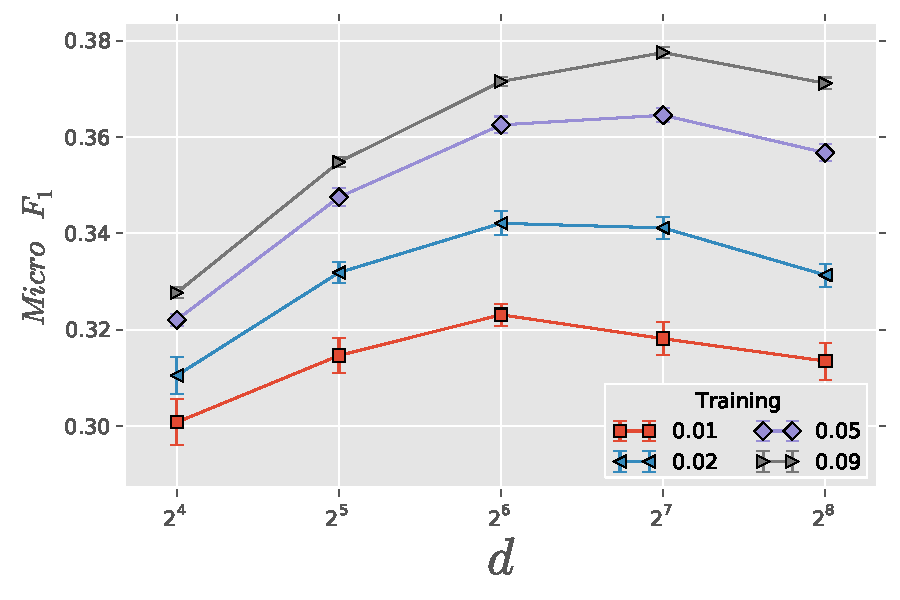
\includegraphics[width=\columnwidth]{figures/stability/flickr_training_vs_dimensions}%
			        \renewcommand\thesubfigure{\alph{subfigure}1}%  	                
	                \caption{\flickr, $\gamma=30$}    	            
    	            \label{fig:stability_flickr-dims_vs_training}
	    	    \end{subfigure}%
	        \begin{subfigure}[b]{0.5\columnwidth}
    		    		\centering	        
	                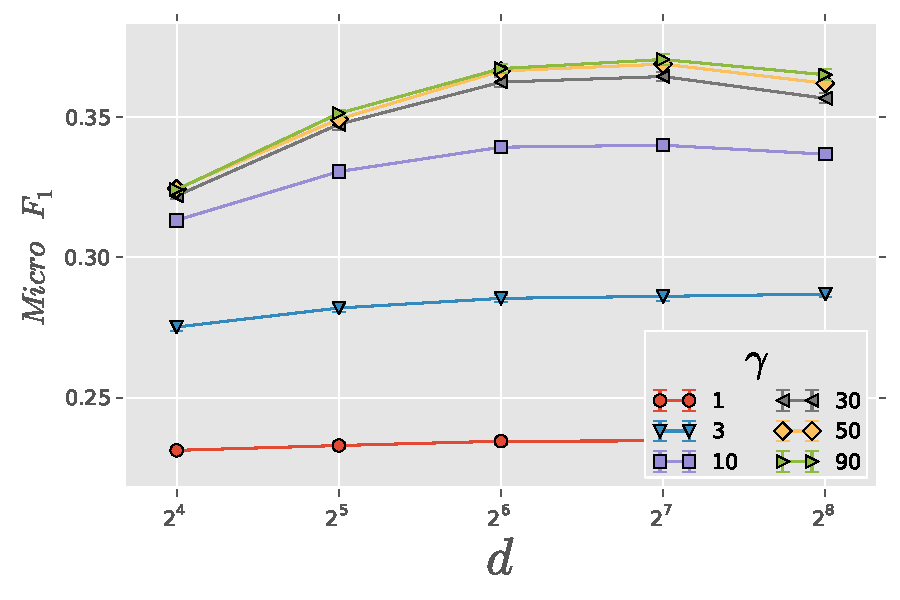
\includegraphics[width=\columnwidth]{figures/stability/flickr_walks_per_node_vs_dimensions}%
				    \addtocounter{subfigure}{-1}%
			        \renewcommand\thesubfigure{\alph{subfigure}2}%  	                
	                \caption{\flickr, $T_R=0.05$}
	                \label{fig:stability_flickr-dims_vs_passes}
	        \end{subfigure}%  	        
%        \addtocounter{subfigure}{-1}
%        \renewcommand\thesubfigure{\alph{subfigure}1}		  
%        \caption{flickr}
%        \label{fig:stability_flickr-dims}
        \end{subfigure}%        
		\hfill
		\begin{subfigure}[b]{\columnwidth} %        
        \begin{subfigure}{0.5\columnwidth} %
                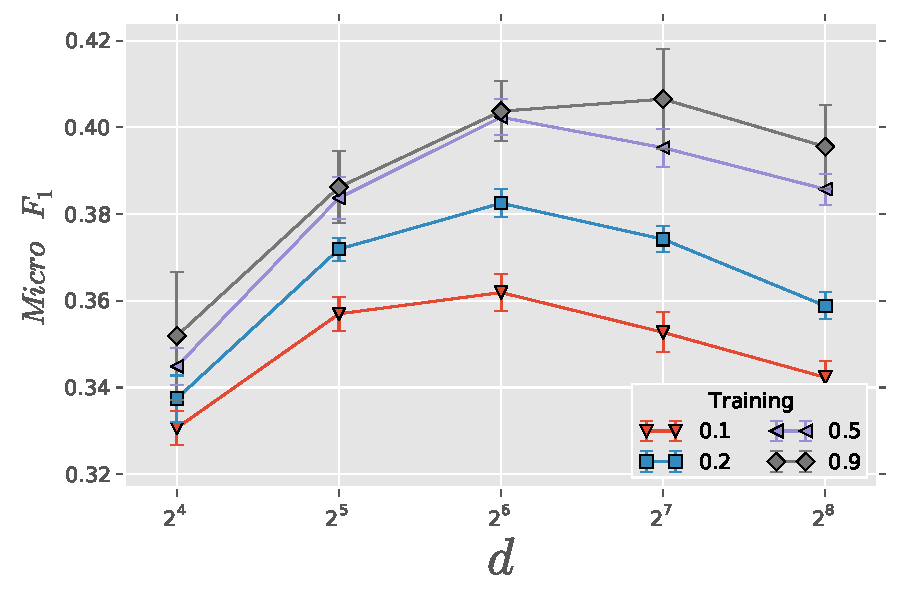
\includegraphics[width=\columnwidth]{figures/stability/blogcatalog_training_vs_dimensions.pdf}%
				    \addtocounter{subfigure}{-1}%
			        \renewcommand\thesubfigure{\alph{subfigure}3}%
	                \caption{\blogcatalog, $\gamma=30$}                
        \label{fig:stability_blogcatalog-dims_vs_training}	                
        \end{subfigure}%
        \begin{subfigure}{0.5\columnwidth}%
                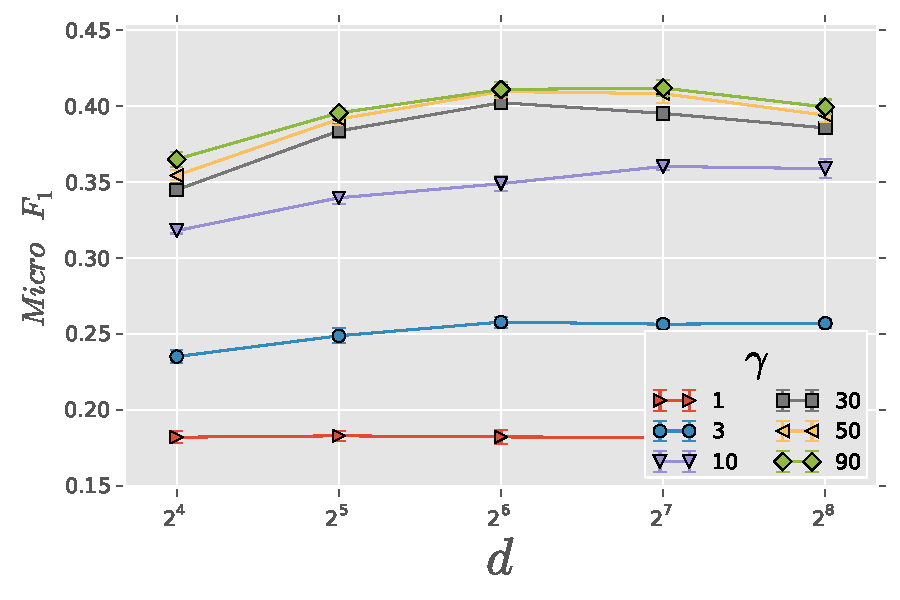
\includegraphics[width=\columnwidth]{figures/stability/blogcatalog_walks_per_node_vs_dimensions.pdf}%
				    \addtocounter{subfigure}{-1}%
			        \renewcommand\thesubfigure{\alph{subfigure}4} %
	                \caption{\blogcatalog, $T_R=0.5$} %
		        \label{fig:stability_blogcatalog-dims_vs_passes}   
        \end{subfigure}        
%        \addtocounter{subfigure}{-1}
%        \renewcommand\thesubfigure{\alph{subfigure}2}                
%        \caption{BlogCatalog}
        \label{fig:stability_blogcatalog-dims}
        \end{subfigure}%               
        \addtocounter{subfigure}{-1}        
		\caption{Stability over dimensions, $d$}
		\label{fig:stability_dimensions}
		\end{subfigure}%     
		\hfill
		%second block, stability over Epochs
		\begin{subfigure}[b]{\columnwidth}			
		\begin{subfigure}[b]{\columnwidth}
    		    \begin{subfigure}[b]{0.5\columnwidth}
    	            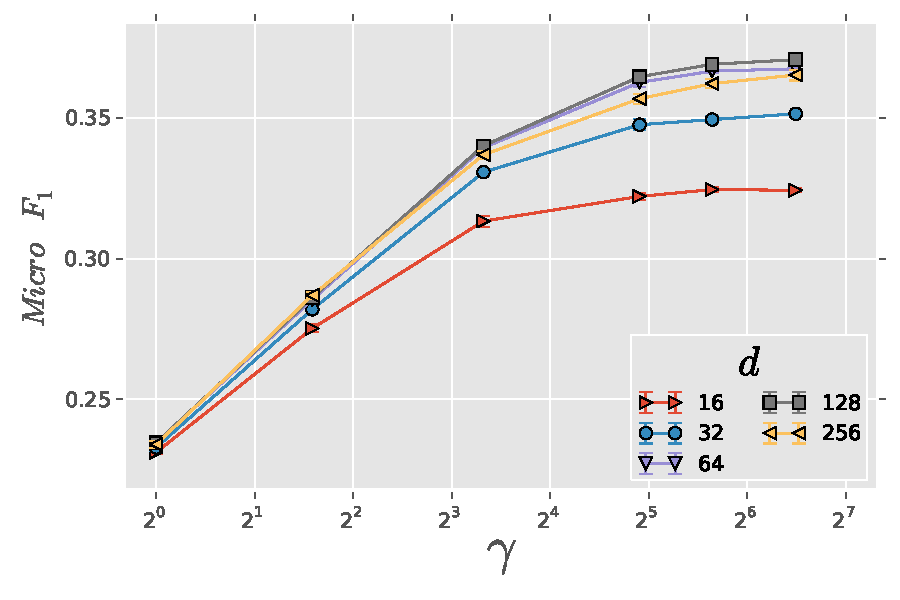
\includegraphics[width=\columnwidth]{figures/stability/flickr_dims_vs_walks_per_node}%
			        \renewcommand\thesubfigure{\alph{subfigure}1}%  	                
	                \caption{\flickr, $T_R=0.05$}    	            
    	            \label{fig:stability_flickr-passes_vs_dims}    	            
	    	    \end{subfigure}%
	        \begin{subfigure}[b]{0.5\columnwidth}
	                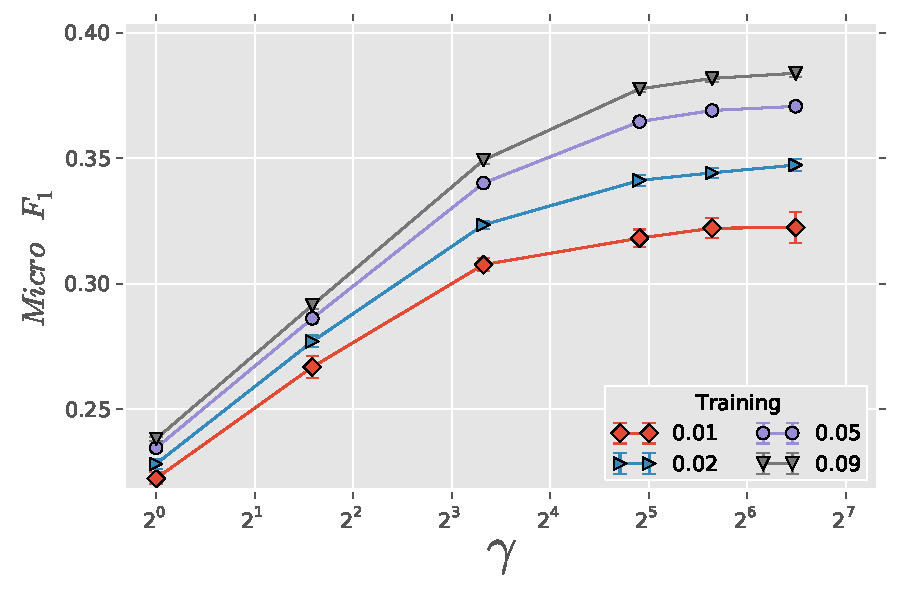
\includegraphics[width=\columnwidth]{figures/stability/flickr_training_vs_walks_per_node}%
				    \addtocounter{subfigure}{-1}%
			        \renewcommand\thesubfigure{\alph{subfigure}2}%  	                
	                \caption{\flickr, $d=128$}
	                \label{fig:stability_flickr-passes_vs_training}	                
	        \end{subfigure}%  	   
%        \renewcommand\thesubfigure{\alph{subfigure}1}		             
%        \caption{flickr}
%        \label{fig:stability_flickr-passes}
        \end{subfigure}%        
		\hfill
		\begin{subfigure}[b]{\columnwidth}        
        \begin{subfigure}{0.5\columnwidth}
                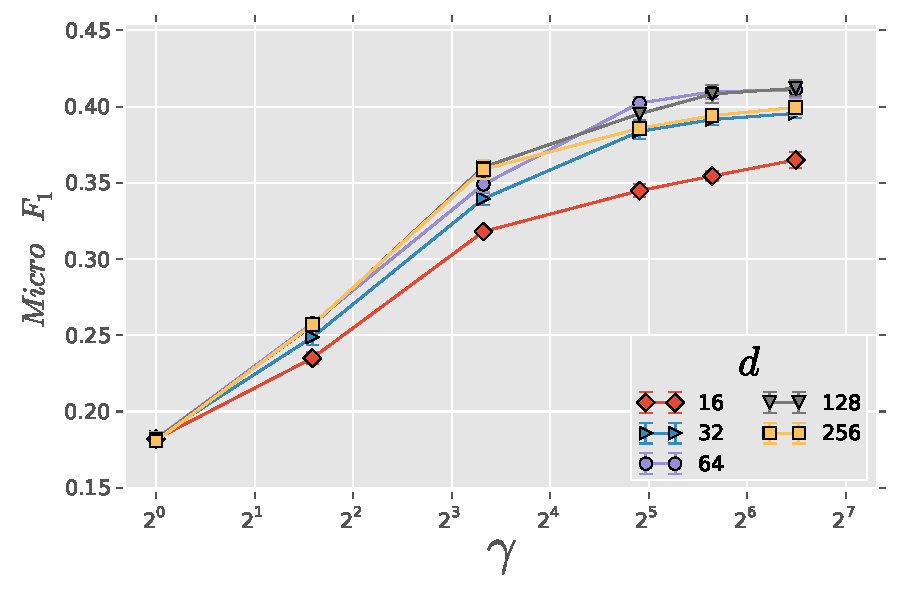
\includegraphics[width=\columnwidth]{figures/stability/blogcatalog_dims_vs_walks_per_node.pdf}%
			    \addtocounter{subfigure}{-1}%
		       \renewcommand\thesubfigure{\alph{subfigure}3}%
               \caption{\blogcatalog,  $T_R=0.5$}                
			   \label{fig:stability_blogcatalog-passes_vs_dims}	                   
        \end{subfigure}%
        \begin{subfigure}{0.5\columnwidth}
                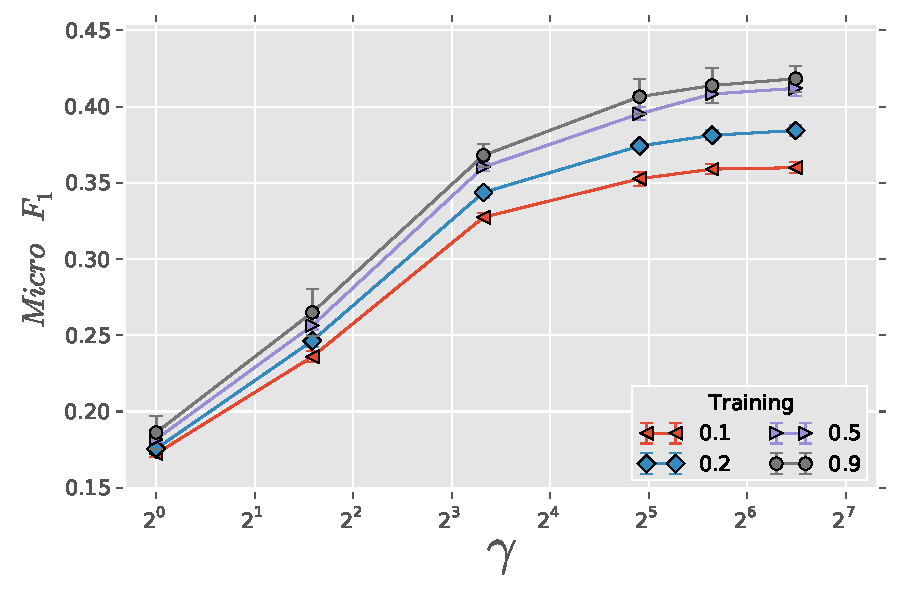
\includegraphics[width=\columnwidth]{figures/stability/blogcatalog_training_vs_walks_per_node.pdf}%
			    \addtocounter{subfigure}{-1}%
		        \renewcommand\thesubfigure{\alph{subfigure}4} %
                \caption{\blogcatalog, $d=128$} %
		        \label{fig:stability_blogcatalog-passes_vs_training}                  
        \end{subfigure}  
        \addtocounter{subfigure}{-1}
%        \renewcommand\thesubfigure{\alph{subfigure}2}                        
%        \caption{BlogCatalog}
%        \label{fig:stability_blogcatalog-passes}		
        \end{subfigure}%    
        \addtocounter{subfigure}{-1}                                 
		\caption{Stability over number of walks, $\gamma$}
		\label{fig:stability_passes}
		\end{subfigure}%                
\caption{Parameter Sensitivity Study}
\label{fig:stability}
\end{figure*}


\subsubsection{Flickr}
In this experiment we vary the training ratio ($T_R$) on the \flickr\ network from 1\% to 10\%.  
This corresponds to having approximately 800 to 8,000 nodes labeled for classification in the entire network. 
Table \ref{tbl:flickr} presents our results, which are consistent with the previous experiment.  \ouralgorithm\ outperforms all baselines by at least 3\% with respect to Micro-$F_1$. 
Additionally, its Micro-$F_1$ performance when only 3\% of the graph is labeled beats all other methods even when they have been given 10\% of the data.
In other words, \ouralgorithm\ can outperform the baselines with 60\% less training data. 
It also performs quite well in Macro-$F_1$, initially performing close to \socdimL, but distancing itself to a 1\% improvement.

\subsubsection{YouTube}
The \youtube\ network is considerably larger than the previous ones we have experimented on, and its size prevents two of our baseline methods (\socdimL\text{} and \socdimB) from running on it.
It is much closer to a real world graph than those we have previously considered.

The results of varying the training ratio ($T_R$) from 1\% to 10\% are presented in Table \ref{tbl:youtube}.
They show that \ouralgorithm\ significantly outperforms the scalable baseline for creating graph representations, \socdimA.  When 1\% of the labeled nodes are used for test, the Micro-$F_1$ improves by 14\%.
The Macro-$F_1$ shows a corresponding 10\% increase.
This lead narrows as the training data increases, but \ouralgorithm\ ends with a 3\% lead in Micro-$F_1$, and an impressive 5\% improvement in Macro-$F_1$.

This experiment showcases the performance benefits that can occur from using social representation learning for multi-label classification.  
\ouralgorithm, can scale to large graphs, and performs exceedingly well in such a sparsely labeled environment.

 

\subsection{Parameter Sensitivity}
In order to evaluate how changes to the parameterization of \ouralgorithm\ effect its performance on classification tasks, we conducted experiments on two multi-label classifications tasks (\flickr, and \blogcatalog).
%In the interest of brevity, we only present the results of one such test here. 
For this test, we have fixed the window size and the walk length to sensible values $(w=10,t=40)$ which should emphasize local structure. 
We then vary the number of latent dimensions ($d$), the number of walks started per vertex ($\mathcal{\gamma}$), and the amount of training data available ($T_R$) to determine their impact on the network classification performance.


\subsubsection{Effect of Dimensionality}
Figure \ref{fig:stability_dimensions} shows the effects of increasing the number of latent dimensions available to our model.

Figures \ref{fig:stability_flickr-dims_vs_training} and \ref{fig:stability_blogcatalog-dims_vs_training} examine the effects of varying the dimensionality and training rate.
The performance is quite consistent between both \flickr\ and \blogcatalog\, and show that the optimal dimensionality for a model is dependent on the number of training examples.  (Note that 1\% of \flickr\ has approximately as many labeled examples as 10\% of \blogcatalog).

Figures \ref{fig:stability_flickr-dims_vs_passes} and \ref{fig:stability_blogcatalog-dims_vs_training} examine the effects of varying the dimensionality and number of walks per vertex.
%Again, the results are generally consistent between the two graphs.
The relative performance between dimensions is relatively stable across different values of $\gamma$.
These charts have two interesting observations.  The first is that there is most of the benefit is accomplished by starting $\gamma = 30$ walks per node in both graphs.
The second is that the relative difference between different values of $\gamma$ is quite consistent between the two graphs.
\flickr\ has an order of magnitude more edges than \blogcatalog, and we find this behavior interesting.

These experiments show that our method can make useful models of various sizes.  They also show that the performance of the model depends on the number of random walks it has seen, and the appropriate dimensionality of the model depends on the training examples available.

\subsubsection{Effect of sampling frequency}
Figure \ref{fig:stability_passes} shows the effects of increasing $\gamma$, the number of random walks that we start from each vertex.  

The results are very consistent for different dimensions (Fig.\ \ref{fig:stability_flickr-passes_vs_dims}, Fig.\ \ref{fig:stability_blogcatalog-passes_vs_dims}) and the amount of training data (Fig.\ \ref{fig:stability_flickr-passes_vs_training}, Fig.\ \ref{fig:stability_blogcatalog-passes_vs_training}).
Initially, increasing $\gamma$ has a big effect in the results, but this effect quickly slows ($\gamma > 10$).
These results demonstrate that we are able to learn meaningful latent representations for vertices after only a small number of random walks.



\comment{
\section{Discussion}
\label{sec:discussion}

\subsection{Why does it work?}

\subsubsection{H1. Random walk is a better way to de-sparsify than PCA on $(A, L, B)$}
Idea:  Machine learning is easier on dense things, and some methods make better dense things

\subsubsection{H2. Decoupling feature space learning from label space avoids cascading errors.}

\subsubsection{H3. Short random walks are enough (partial topology)}

\subsubsection{H4. Plotting these things in 2-D will reveal differences on Cora}

\subsection{Limitations}
\todo{Improve this}
\subsubsection{Homophily Assumption}
Using random walks to extract information from graphs places limits on the type of information that we can hope to extract from the network.
Specifically, random walk methods have a strong homophily assumption, expecting that random walk distance is correlated in some way with the output space.
While this assumption holds in many real world in many real-world graphs, it might not be a good assumption in some (e.g. in bipartite networks \cite{Gallagher:2008:UGE:1401890.1401925}).
This emphasis on homophily also means that random walk methods can not effectively capture heterophily as some relational classification approaches can \cite{neville2000iterative}.

\subsubsection{Scale}
The largest correlations we can hope to model are limited by the length of the window.
}

\section{Related Work}
\label{sec:related}
The main differences between our proposed method and previous work can be summarized as follows: 
\begin{enumerate} [itemsep=0pt, topsep=5pt, partopsep=0pt]
\item We \emph{learn} our latent social representations, instead of computing statistics related to centrality \cite{gallagher2010leveraging} or partitioning \cite{Tang:2011:Leveraging}.
\item We do not attempt to extend the classification procedure itself (through collective inference \cite{sen2008collective} or graph kernels \cite{kondor2002diffusion}).
\item We propose a scalable online method which uses only local information.  Most methods require global information and are offline \cite{Tang:2009:RLV:1557019.1557109,tang2009scalable,Tang:2011:Leveraging,Henderson:2011:YKG:2020408.2020512}.
\item We apply unsupervised representation learning to graphs.
\end{enumerate}
In this section we discuss related work in network classification and unsupervised feature learning.

\subsection{Relational Learning}
Relational classification (or \emph{collective classification}) methods \cite{Macskassy03asimple,neville2000iterative,Pearl:1988:PRI:534975,geman1984stochastic} use links between data items as part of the classification process. 
Exact inference in the collective classification problem is NP-hard, and solutions have focused on the use of approximate inference algorithm which may not be guaranteed to converge \cite{sen2008collective}.

The most relevant relational classification algorithms to our work incorporate community information by learning clusters \cite{Neville:2005:LRA:1090193.1090201},  by adding edges between nearby nodes \cite{Gallagher:2008:UGE:1401890.1401925}, by using PageRank \cite{cohenASOM}, or by extending relational classification to take additional features into account \cite{wang2013multi}.
Our work takes a substantially different approach.  
Instead of a new approximation inference algorithm, we propose a procedure which learns representations of network structure which can then be used by existing inference procedure (including iterative ones).  

A number of techniques for generating features from graphs have also been proposed \cite{gallagher2010leveraging,Tang:2009:RLV:1557019.1557109,tang2009scalable,Tang:2011:Leveraging,Henderson:2011:YKG:2020408.2020512}.
In contrast to these methods, we frame the feature creation procedure as a representation learning problem.

Graph Kernels \cite{vishwanathan2010graph} have been proposed as a way to use relational data as part of the classification process, but are quite slow unless approximated \cite{kang2012fast}.  
Our approach is complementary;  instead of encoding the structure as part of a kernel function, we learn a representation which allows them to be used directly as features for any classification method.

\subsection{Unsupervised Feature Learning}
Distributed representations have been proposed to model structural relationship between concepts \cite{distributed}.
These representations are trained by the back-propagation and gradient descent.
Computational costs and numerical instability led to these techniques to be abandoned for almost a decade.
Recently, distributed computing allowed for larger models to be trained \cite{nnlm}, and the growth of data for unsupervised learning algorithms to emerge \cite{erhanhelps}.
Distributed representations usually are trained through neural networks, these networks have made advancements in diverse fields such as computer vision \cite{vision1}, speech recognition \cite{speech1}, and natural language processing \cite{senna1}.


\section{Conclusions}
\label{sec:conclusion}
We propose \ouralgorithm, a novel approach for learning latent social representations of vertices. 
Using local information from truncated random walks as input, our method learns a representation which encodes structural regularities.
Experiments on a variety of different graphs illustrate the effectiveness of our approach on challenging multi-label classification tasks.

As an online algorithm, \ouralgorithm\textsc{} is also scalable. Our results show that we can create meaningful representations for graphs too large to run spectral methods on.
On such large graphs, our method significantly outperforms other methods designed to operate for sparsity.
We also show that our approach is parallelizable, allowing workers to update different parts of the model concurrently.

In addition to being effective and scalable, our approach is also an appealing generalization of language modeling. 
This connection is mutually beneficial.  
%We hope for a continued connection between the fields.  
Advances in language modeling may continue to generate improved latent representations for networks.
In our view, language modeling is actually sampling from an unobservable language graph.  We believe that insights obtained from modeling observable graphs may in turn yield improvements to modeling unobservable ones.

Our future work in the area will focus on investigating this duality further, using our results to improve language modeling, and strengthening the theoretical justifications of the method.


\bibliography{paper}
\bibliographystyle{abbrv}

\end{document}



